\documentclass{ntuthesis}

\usepackage{times}
\usepackage{verbatim}
\usepackage{color}
\usepackage{url}
\usepackage{graphicx}
\usepackage{array}
\usepackage{wallpaper} 

% Additional packages
\usepackage[vlined, ruled]{algorithm2e}
\usepackage{multirow}
\usepackage{amsmath}
\usepackage{bm}
\usepackage{lmodern}
\usepackage{booktabs} % For formal tables


% Using the tex-text mapping for ligatures etc.
\defaultfontfeatures{Mapping=tex-text}

% Set the default fonts
\setmainfont{Times New Roman}
\setCJKmainfont{標楷體}

\ifdefined\withwatermark
  \CenterWallPaper{0.174}{watermark.pdf}
  \setlength{\wpXoffset}{6.1725cm}
  \setlength{\wpYoffset}{10.5225cm}
\fi

% Your information goes here
% author: Tz-Huan Huang [http://www.csie.ntu.edu.tw/~tzhuan]

% ----------------------------------------------------------------------------
% "THE CHOCOLATE-WARE LICENSE":
% Tz-Huan Huang wrote this file. As long as you retain this notice you
% can do whatever you want with this stuff. If we meet some day, and you think
% this stuff is worth it, you can buy me a chocolate in return Tz-Huan Huang
% ----------------------------------------------------------------------------

% Syntax: \var{English}{Chinese}
\university{National Taiwan University}{國立臺灣大學}
\college{College of Electrical Engineering and Computer Science}{電機資訊學院}
\institute{Department of Electrical Engineering}{電機工程學系}
\title{Real-valued Optimization by Subspace Projection and Multi-armed Bandit Techniques}
{基於子空間映射與多臂吃角子老虎機技術之\\實數最佳化}
\author{Chun-Jen Peng}{彭俊人}
\studentid{R04921039}
\advisor{Tian-Li Yu, Ph.D.}{于天立 博士}
\defenseyear{2017}{106}
\defensemonth{July}{7}
\defenseday{28}


\begin{document}

\frontmatter

\makecover

\makecertification

\begin{acknowledgementszh}
感謝徐世曦在我人生苦悶時聽我發牢騷,順到給我許多研究上的建議
感謝我弟弟彭俊又時常忍受我對研究問題的碎碎念,幫助我釐清思緒\ldots
\end{acknowledgementszh}

\begin{acknowledgementsen}
I'm glad to thank\ldots 
\end{acknowledgementsen}

\begin{abstractzh}
本論文提出了一新的實數多模態(multimodal)最佳化方法。
大多數的現實問題都可以由多個單峰問題合成。
而對於實數最佳化,我們較感興趣的是多模態且可被拆解成多個階層化的單峰問題。
然而,一旦面對多模態問題,我們就必須面對利用性(exploitation)與探索性(exploration)的問題。
本論文提出一解決多模態問題的技巧。
此技巧結合了階層式聚合(hierarchically clustering)與最小描述長度(minimum description length), 來辨識搜尋空間中可能的單峰模型。
接著,我們使用一加一演化策略((1+1)-Evolutionary Strategy)來最佳化一齊次座標(homogeneous coordinate)上的線性轉換矩陣,
並利用此矩陣將原搜尋空間投影到另一有良好邊界定義的子空間。
此投影嘗試定義出只包含一單峰之感興趣區域(region of interest)。
最後,我們提出一新的多臂吃角子老虎(multi-armed bandit)技術,
來分配給各個子空間的資源,以最大化獲得全域最佳解的機率,
我們將此結果與自適應共變異數矩陣演化策略(Covariance Matrix Adaptation Evolution Strategies, CMA-ES)、
標準粒子群演算法(Standard Particle Swarm Optimization 2011)、
與實數域蟻群演算法(Ant Colony Optimization for Continuous Domain, ACO$_R$)結合,
並利用CEC 2005實數最佳化測試問題來比較結果。
\end{abstractzh}

\begin{abstracten}
This thesis presents a new technique for real-valued multimodal optimization.
Most of the real-world problems can be described as a composition of unimodal subproblems.
For real-valued optimization, we are interested in problems that are composed of \textit{multiple hierarchically decomposable} unimodals.
However, allocating resources to exploit different unimodals leads to the 
common dilemma between \textit{exploration} and \textit{exploitation}.
This thesis proposed some new techniques that aim to solve multimodal problems more efficiently.
A new technique combining hierarchical clustering and minimum description length (MDL) 
is proposed to help identify potential unimodals in the search space.
Then, a linear transform matrix in homogeneous coordinate, optimized by the (1+1)-Evolutionary Strategy,
projects the search space to a subspace with well-defined boundary.
This projection aims to define a region of interest (ROI) that isolates a unimodal subproblem.
Finally, a new multi-armed bandit technique, aiming to maximize the probability of acquiring the global optimum,
is proposed to allocate resources for each unimodal.
We combined our new techniques with Covariance Matrix Adaptation Evolution Strategy (CMA-ES), 
Standard Particle Swarm Optimization (SPSO) 2011, and Ant Colony Optimization for Continuous Domain (ACO$_R$).
The results are evaluated with the CEC2005 Special Session on Real-Parameter Optimization benchmark problems.
\end{abstracten}

\begin{comment}
\category{I2.10}{Computing Methodologies}
{Artificial Intelligence -- Vision and Scene Understanding} 
\category{H5.3}{Information Systems}
{Information Interfaces and Presentation (HCI) -- Web-based Interaction.}

\terms{Design, Human factors, Performance.}

\keywords{Real-valued Optimization, Multimodal Optimization, Homogeneous Coordinates, Multi-armed Bandit Algorithm.}
\end{comment}


\tableofcontents
\listoffigures
\listoftables

\mainmatter

% Your thesis goes here
\chapter{Introduction}
\label{c:intro}

% Background, Motivation and Relevant work
Multimodal problems that contain more than one region or more than one local optimum are common in the real world.
{\em Rastrigin function}, a hierachical problem which is composed of a larger hill and multiple smaller hills are also well-known in real-valued optimization.
In order to tackle these multimodal problems with a limited amount of resources, 
one needs to decide how much to invest for searching a better hill, 
while still maintain enough of exploitation on each potential hill.

The difficult part is that searching for a new hill and exploiting the best hill often require opposite searching behaviors.
For a fixed amount of total evaluations, spending more time searching on one hill implies 
less attention on exploring other possible unimodals in the search space.
This is the common dilemma between {\em exploration} and {\em exploitation} for real-valued optimization algorithms.
Also, during different phases of optimization, 
the ratio between exploring new hills and exploiting the current best hill should be altered.
Exploration is more important in the beginning, while exploitation is more required in the end.
What makes this problem even harder is that in order to decrease the number of total evaluations, 
the size of the population are often limited in the real-valed optimization algorithms.
This means that as the number of hills to invest increases, the number of particles on each hill decreases.
This weakens the exploitation ability on each hill, making it less likely to identify new potential regions on each hill.

We are more interested in hierarchically decomposable problems.
With a certain amount of hints, we should be able to focus on one of the many potential hills, 
and identify when to invest more on certain hills to iteratively discover more smaller hills.
Also, we would like to only focus on some regions instead of the whole search spaces, in order to gain performance.
This requires detection of promising areas, and search space splitting techniques.
Moreover, after identifying certain interesting regions, we also need to decide how to allocate our resources.
Given the abilities described above, 
we can pay more attention on the promising regions and 
iteratively break down a difficult multimodal problem into smaller and easier unimodal problems.

% Thesis Objective
\section{Thesis Objectives}
We propose some techniques to break down multimodal problems into several unimodal problems in smaller non-overlapping subspaces.
We believe that solving one unimodal problem on a smaller subspace is easier than tackling the complete search space as a whole.
This technique can \textbf{identify potential unimodal},
\textbf{define a region of interest} to exploit, 
and \textbf{allocate resources} according to remaining evaluations.

Identifying a \textit{unimodal} depends on the sampling frequency and the underlying model.
Clustering is a common way for discovering potentail unimodals.
We adopt the hierarchical clustering technique to discover hills in the fitness landscape.
We also use weighted normal distribution as the underlying consumption for unimodal, and trim overfitting models with minimum description length.

After identifying the unimodals by clustering, we can split the search space into different regions of interest with linear projection.
We use different projection matrices to project the original search space onto several subspaces with well-defined boundaries.
We also optimize the porjection matrix so that each region would have minimum overlapping with others.
Searching in the smaller subspace enhances the probability of finding optimium.
The well-defined boundaries are also needed for some algorithms.
The projection might also rotate or shear the original search space, making some inseparable problems easier to solve.

With multiple subspace to search, we propose a new Multi-armed Bandit (MAB) technique 
that optimize the resource allocation to get the greatest probability of obtaining the global optimum.
Multi-armed Bandit algorithms are suitable for this scenario, 
since it learns models from outcomes while the actions do not change the state of the world.
When there are still plenty of evaluations left, we should prefer exploration over exploitation and search equally on all subspaces.
However, when few evaluations remain, we should focus on the current best hill 
and try to exploit it to get the best fitness with the remaining evaluations.  


\section{Roadmap}
This thesis is composed of eight chapters.

\textbf{Chapter~\ref{chapter:algos}} presents three optimization algorithms that are used for comparisons.
We introduce 
the Covariance Matrix Adaptation Evolutionary Strategy (CMA-ES),
the Standard Particle Swarm Optimization, and
the Ant Colony Optimization for Continous Domain.
These three algorithms each have different characteristics due to different underlying models.


\textbf{Chapter~\ref{chapter:clustering}} presents some clustering techniques that guides the construction of ROIs and later becomes the initial points for algorithms in each arm.  

\textbf{Chapter~\ref{chapter:projection}} first describes four basic affine transformation: translation, rotation, scaling and shearing.
Then the projective transformation and homogeneous coordinate are presented.


\textbf{Chapter~\ref{chapter:MAB}} first describes the Multi-armed Bandit Algorithm, 
followed by a brief introduction of some common MAB algorithms, including ...
Then we present our new bandit techniques.
Tranditional bandit algorithms focus on minimizing regret, while our new bandit focus on the probability of getting a rank 1 result.


\textbf{Chapter~\ref{chapter:new_bandit}} gives details of our new algorithms.
First, the framework and pseudo code are given.
Then a detailed process of initialization is given in ...
% talk about ROI, what it is, why it is important

\textbf{Chapter~\ref{chapter:conclusion}} summarizes this thesis. 
The conclusion and contributions are also given.
Some further improvements and future works are also discussed at the end.



\chapter{Real-valued Optimization Algorithms}
\label{chapter:algos}

Overview of real-valued optimization

\section{Covariance Matrix Adaptation Evolution Strategy}

Describe history of \textit{Evolutionary Strategies} (ES).
The simplest algorithm is (1+1)-ES.
Here we describe the (1+1)-ES with one-fifth success rule with independent restarts.
The pseudo code of (1+1)-ES is given in Algorithm~\ref{algo:1+1ES}.

Covariance Matrix Adaptation Evolution Strategy (CMA-ES) is an extended version fo CSA-ES with de-randomized adaptation of covariance matrix.
Describe the underlying covariance matrix model.

Describe how to update \textit{mean}.

Describe how to update \textit{covariance matrix}.

Describe \textit{step-size} control.



\begin{algorithm}%[t!]
\caption{(1+1)-ES with 1/5 success-rule}\label{algo:1+1ES}

$\boldsymbol{X}_{n}$: solution of the $n^{th}$ iteration, $\sigma_n$: step size of the $n^{th}$ iteration, \\
$N(\boldsymbol{0}, \boldsymbol{I})$: multivariant normal distribution with mean vector $\boldsymbol{0}$ \\ 
and identical covariance matrix $\boldsymbol{I}$.

\BlankLine
\SetKwInOut{Input}{input} \SetKwInOut{Output}{output}
\Input{ $f$: evaluation function }
\Output{ $X_{n+1}$: best solution }

\BlankLine
Initialize $\boldsymbol{X}_0, \sigma_0$ \\
\While{ termination criterion not met } {

    $\widetilde{\boldsymbol{X}}_n = \boldsymbol{X}_n + \sigma_n N(\boldsymbol{0}, \boldsymbol{I})$  \\

    \eIf{ $f(\widetilde{\boldsymbol{X}}_n) \leq f(\boldsymbol{X}_n) $}{
        $\boldsymbol{X}_{n+1} = \widetilde{\boldsymbol{X}}_n$ \\
        $\sigma_{n+1} = 1.5 \sigma_n$
    }{
        $\boldsymbol{X}_{n+1} = \boldsymbol{X}_n$ \\
        $\sigma_{n+1} = 1.5^{-1/4}\sigma_n$
    }
}

\Return $\boldsymbol{X}_{n+1}$

\end{algorithm}





\section{Standard Particle Swarm Optimization}

Particle Swarm Optimization was first proposed by ...
The swarm intelligence family... 
However, there are multiple varients of PSO over the years.

Standard PSO provides a well defined version of PSO that follows the basic principles.
It is intend to be a milestone for future comparison, instead of the best algorithm on the market.

So far, there have been three successive versions of standard PSO: SPSO 2006, 2007 and 2011
The underlying principles of these three versions are generally the same as all PSO varients.
The exact formula and implementation are slightly different due to latest theoretical progress.

Describe swarm size definition and basic elements for each particle.
Initialization of the swarm.
The swarm size, denoted as $S$, differs in SPSO 2006 and SPSO 2011.
In both SPSO 2006 and SPSO 2007, the initial number of particles for dimension $D$ is defined as:
\begin{displaymath}
S = 10 + \lfloor 2\sqrt{D} \rfloor,
\end{displaymath}
However, in SPSO 2011, the swarm size can be defined by user, yet suggested as 40~\cite{Clerc:2012:SPSO2011} since the original swarm size is far from optimal.

Each particle in the swarm possesses the following elements: current position, current velocity, personal pervious best position, and previous best position in the neighbourhood. 


Describe random topology and when to update topology.
The information links...
The adaptive random topology described in ~\cite{Clerc:2007:randomTopology} is formally equivalent to "Stocastic Star".

Describe velocity update for SPSO 2006 and SPSO 2011
Update Velocity as shown in Figure~\ref{fig:SPSO_update}
\begin{figure}
\centering
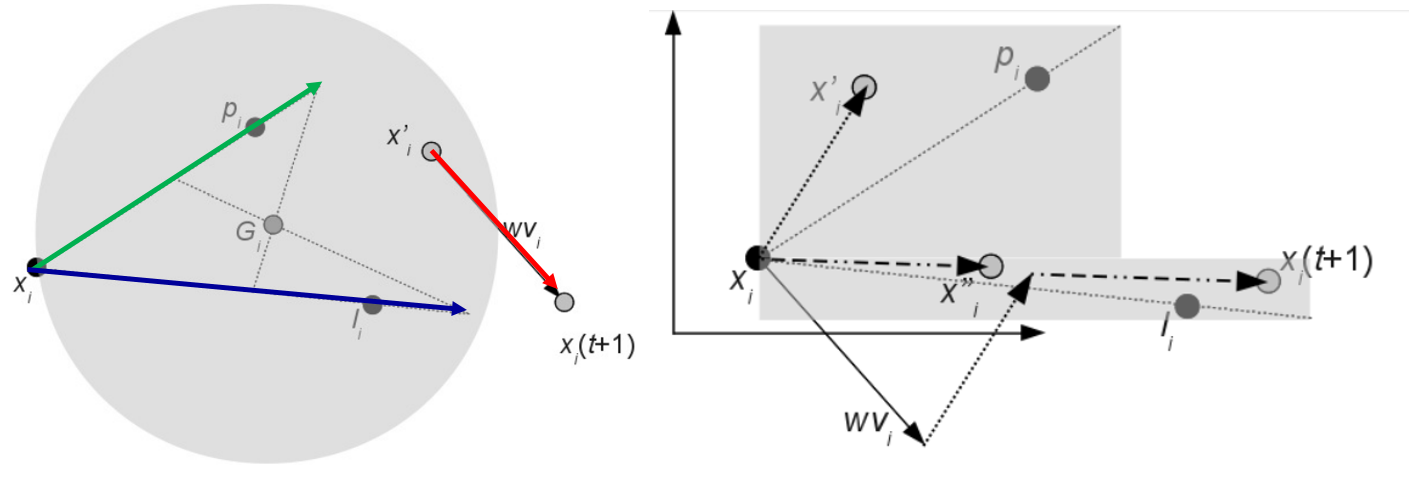
\includegraphics[width=\textwidth]{SPSO_update}
\caption{(a) SPSO 2011. (b) SPSO 2006.}\label{fig:SPSO_update}
\end{figure}

Describe boundary and out-of-bound handling.



The pseudo code defined in~\cite{Zambrano:2013:SPSO2011}.
The pseudo code is given in Algorithm~\ref{algo:SPSO2011}.



\begin{algorithm}%[t!]
\caption{Standard PSO 2011}\label{algo:SPSO2011}

$\boldsymbol{X}_{n}$: solution of the $n^{th}$ iteration, $\sigma_n$: step size of the $n^{th}$ iteration, \\
$N(\boldsymbol{0}, \boldsymbol{I})$: multivariant normal distribution with mean vector $\boldsymbol{0}$ \\ 
and identical covariance matrix $\boldsymbol{I}$.

\BlankLine
\SetKwInOut{Input}{input} \SetKwInOut{Output}{output}
\Input{ $f$: evaluation function }
\Output{ $X_{n+1}$: best solution }

\BlankLine
Initialize $\boldsymbol{X}_0, \sigma_0$ \\
\While{ termination criterion not met } {

    $\widetilde{\boldsymbol{X}}_n = \boldsymbol{X}_n + \sigma_n N(\boldsymbol{0}, \boldsymbol{I})$  \\

    \eIf{ $f(\widetilde{\boldsymbol{X}}_n) \leq f(\boldsymbol{X}_n) $}{
        $\boldsymbol{X}_{n+1} = \widetilde{\boldsymbol{X}}_n$ \\
        $\sigma_{n+1} = 1.5 \sigma_n$
    }{
        $\boldsymbol{X}_{n+1} = \boldsymbol{X}_n$ \\
        $\sigma_{n+1} = 1.5^{-1/4}\sigma_n$
    }
}

\Return $\boldsymbol{X}_{n+1}$

\end{algorithm}




\section{Ant Colony Optimization for Continuous Domain}

Ant Colony optimization (ACO) is first proposed by Dorigo~\cite{Dorigo:1999:ACO} to solve combinatorial optimization problems, including scheduling, routing, and timetabling.
These problems aim to find optimal \textit{combinations} or \textit{permutations} of finit sets of available components.
Inspired by the foraging behavior of natural ants, ACO mimics the pheromone deposition of ants along the trail to a food source.
The deposited pheromone, which indicates the quantity and quality of the food, creates an indirect communication among ants and enables them to find the shortest paths.
The pseudo code of ACO is given in Algorithm~\ref{algo:ACO}.
Two major procedures: \textit{solution construction} and \textit{phermone update}, are detailed in the following paragraph.


Consider a search space $\boldsymbol{S}$ defined over a finit set of all possible \textit{solution components}, denoted by $\boldsymbol{C}$.
Each solution component, denoted by $c_{ij}$, is a decision variable $X_i$ instantiated with value $v^{j}_{i} \in \boldsymbol{D}_i = \{ v^{1}_{i}, ..., v^{|\boldsymbol{D}_i|}_{i}\}$.
To construct a new solution, an artificial ants starts with an empty partial solution $s^{p} = \emptyset$.
During each construction step, the partial solution $s^{p}$ is extended with a feasible solution from the set $N(s^{p}) \in \boldsymbol{C} \setminus s^{p}$.
The probabilistic pheromone model adopted for selecting a feasible solution from $N(s^{p})$ can be defined as follows:

\begin{equation}
p(c_{ij}|s^p) = \frac{\tau^{\alpha}_{ij} \cdot \eta(c_{ij})^{\beta}} 
                     {\sum_{c_{i\ell}\in N(s^{p})} \tau^{\alpha}_{i\ell} \cdot \eta(c_{i\ell})^{\beta} },  \forall c_{ij} \in N(s^{p}),
\end{equation}
where $\tau_{ij}$ is the pheromone value associated with component $c_{ij}$, and $\eta(\cdot)$ is a weighting function. 
% that assigns at each construction step a heuristic value to each feasible solution component $c_{ij} \in N(s^{p})$.
$\alpha$ and $\beta$ are positive parameters which determine the relation between phermone and heuristic information.

The pheromone update


Over the years, multiple approaches of extending the ACO on continous domain have been given.
One of the most successful version is ACO$_{R}$, proposed by Socha and Dorigo in 2008~\cite{Socha:2008:ACOR}.
It extends ACO to the continuous domain without making any major conceptual change to its structure.
The fundamental idea underlying ACO$_{R}$ is the shift from using a discrete probability distribution to using a continuous one, demonstrated in Figure~\ref{fig:ACOR_distribution}. 

A enhanced Gaussian kernel PDF as shown in Figure~\ref{fig:ACOR_gaussianKernel}.

\begin{figure}
\centering
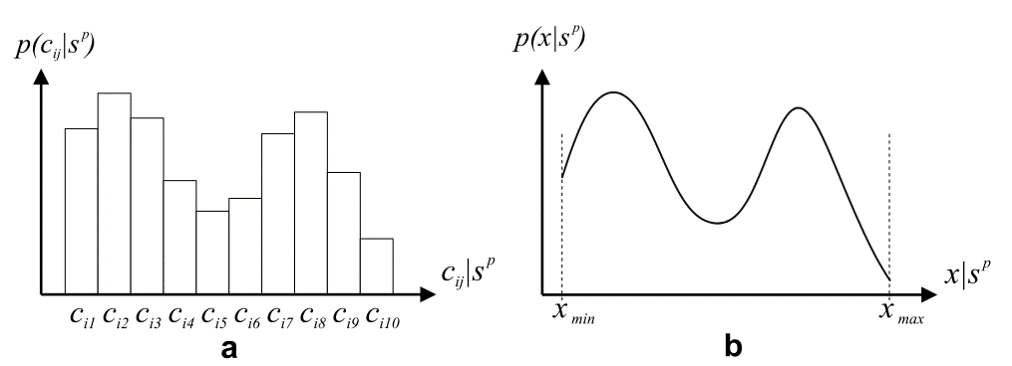
\includegraphics[width=\textwidth]{ACOR_distribution}
\caption{(a) Discrete probability distribution $p(c_{ij}|s^{p})$. (b) Continuous probability density function $p(x|s^{p})$}\label{fig:ACOR_distribution}
\end{figure}

\begin{figure}
\centering
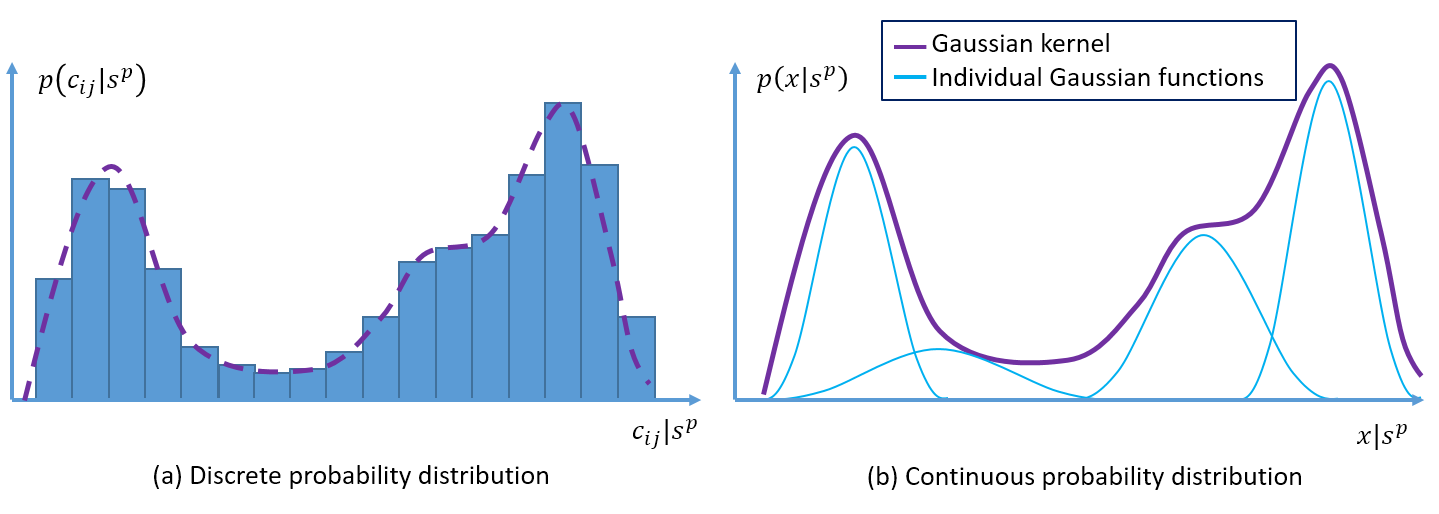
\includegraphics[width=\textwidth]{ACOR_gaussianKernel}
\caption{(a) Discrete probability distribution $p(c_{ij}|s^{p})$. (b) Continuous probability density function $p(x|s^{p})$}\label{fig:ACOR_gaussianKernel}
\end{figure}

\begin{algorithm}%[t!]
\caption{Ant Colony Optimization metaheuristic}\label{algo:ACO}
\While{ termination criterion not met } {

    schedule activities \\
    solution contruction by ants(); \\
    phermone update(); \\
    daemon actions(); \\
}
\end{algorithm}




\chapter{Clustering Techniques}
\label{chapter:clustering}

%Describe our basic assumption of function decomposition.
%Each subproblem should be composed of an observalbe unimodel.
We are interested in solving real-valued multimodal problems composed of observable unimodals.
Given the case, it is easier to solve an isolated unimodal within a subspace,
than tackling the complete search space with the multimodal problem.
Therefore, the first thing for solving a multimodal problem is to \textbf{identify} and \textbf{isolate}
the potential unimodals within the given search space.

%We wish to identify these unimodels through clustering techniques. 
We tried to isolate potential \textit{fitness hills}, \textit{i.e.} unimodals,
by \textbf{clustering} the initial samples points,
and consider each cluster as a multi-dimension normal distribution.
Different clustering techniques are often applied to identify different characteristics of clusters.
Here we proposed a \textit{hierarchical clustering} techniques to identify \textit{fitness hills},
since we consider not only the density of the particles,
but also the fitness values of different search points.
Our basic assumption for the under lying unimodal is a weighted normal distribution, 
since we need to take fitness into account instead of viewing each point with the same weight.
We tend to focus on the particles with better fitness,
than a dense cluster with less fitness. 
It is also easier to calculate the weighted mean vector and weighted covariance matrix in higher dimension. 

Later, we applied the \textbf{Minimum Description Length} (MDL) to reduce the number of clusters.
Although a complex Gaussian Mixture Modal is able to describe the sample distribution better,
we believe that a more compact model, in terms of information entropy, is the better choice 
when multiple models can describe the same distribution. 
This also allows us to define a more stable subspace for further searching.


\section{K-Means Clustering}
In this section, we first describe the K-Means clustering techniques and its limitation for identifying the fitness hills.
K-Means clustering aims to partition $n$ observation data points into $k$ clusters.
There are two main procedures for K-Means clustering: the \textit{assignment} step and the \textit{update} step.

During the \textit{assignment} step, an initial set of $k$ means positions are given.
Then, each data point is assigned to the cluster with the \textit{nearest mean}.
The assignment to the \textit{nearest mean} can be formally described 
as creating clusters whose mean yields the least within-cluster sum of squares (WCSS), textit{i.e.} the sum of squared Euclidean distance.
During the \textit{update} step, the new centroids of each new clusters are calculated and assigned as the new means.
This can be also be described as minimizing the WCSS.
The algorithm proceeds by alternating between these two steps until the means no longer change.
Since there only exists a finite states of partitions, the algorithm must converge to a local optimum.
However, different initial mean positions results in different clusters.

One of the main problem for using the K-Means clustering to identify \textit{fitness hills} is that
it considers only the \textit{spatial density} and does not utilize the fitness value of each particle.
Different sets of initial centers might result in different kinds of clusters.
Meanwhile, each cluster might be centering at a point that does not necessarily possess the best fitness in the neighborhood.
Therefore, the K-Means clustering often results in \textbf{unstable clusters} depending on initial conditions, and is highly sensitive to particle density.
Another common phenomenon for being sensitive to spatial density is that 
the points on the \textit{border of clusters} might belong to different clusters after each update.
This makes the clusters unstable and costs unnecessary evaluations and computation for redefining the borders of ROI after each update. 

The other problem for using the K-Means clustering is that one needs to \textbf{decide the number of clusters}.
Determining the number of clusters is also a highly studied subjects.
We briefly discuss three common estimation methods that we have tried, 
the \textit{silhouette coefficient}~\cite{Rousseeuw:1987:silhouettes}
, the \textit{gap statistics}~\cite{Tibshirani:2001:gap}
, and the \textit{Hartigans' dip test}~\cite{Hartigan:1985:dip}
in the following paragraph.

The \textit{silhouette coefficient} measures how cohesive an object is to its own cluster and how separated it is to the other clusters. Ranging from -1 to 1, the silhouette coefficient with a higher value indicates it is more likely to belong to its own cluster.
The \textit{gap statistics} compares the change in within-cluster dispersion with that of an reference null distribution.
It calculates the gap statistics for different number of clusters and select the one with the maximum gap statistics.
The \textit{Hartigans' dip test} uses the empirical cumulative distribution function (ECDF) to measure the maximum difference between multimodal samples and the unimodal samples. It calculates maximum deviation of the sample ECDF from the unimodal CDF and check if the difference is statistically significant.


We desire that as the algorithms proceed, particles should gather around the good solutions and gives a clear density signal.
However, they seldom identify a unimodal at the beginning.
It means that we need to add up more particles to meet the population size requirement for each clusters.
This increases the density in that specific region, and creates an artificial cluster that should not exist in the first place.

\begin{figure} 
\centering
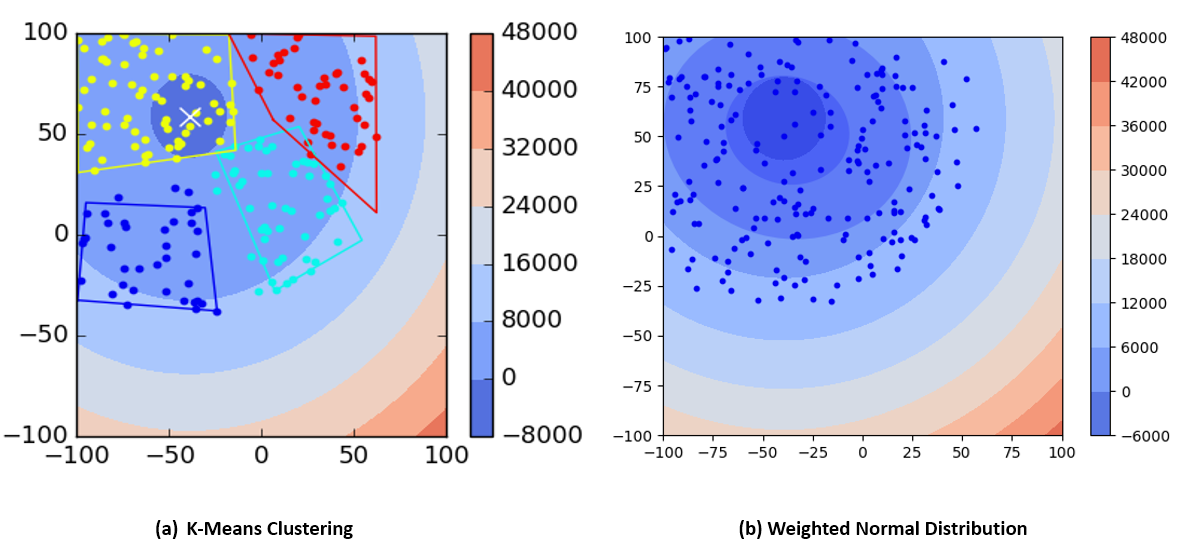
\includegraphics[width=\textwidth]{Clustering_comparison} 
\caption{Comparing K-Means clustering with weighted Gaussian Distribution on CEC2005 F1 Problem}\label{fig:Clustering_comparison}
\end{figure}

Figure~\ref{fig:Clustering_comparison} shows how K-Means fails to identify a unimodal and results in four clusters due to density.
A more preferable clustering result is shown on the right in Figure~\ref{fig:Clustering_comparison}.
We would like our clustering method to be capable of identifying the unimodal 
and be able to center around the particle with the best fitness.

\begin{figure}
\centering
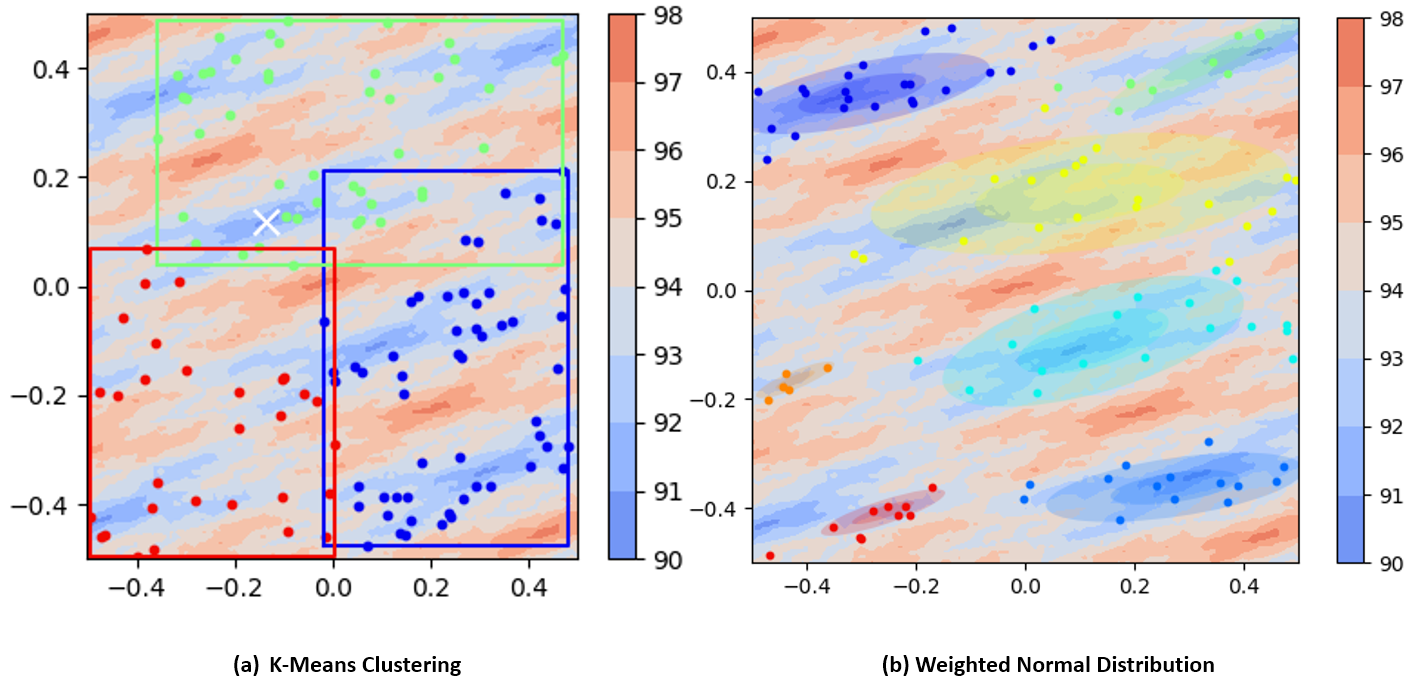
\includegraphics[width=\textwidth]{Clustering_comparison_F11}
\caption{Comparing K-Means clustering with weighted Gaussian Distribution on CEC2005 F11 Problem}\label{fig:Clustering_comparison_F11}
\end{figure}

Figure~\ref{fig:Clustering_comparison_F11} shows another example of how K-Means fails to identify the right multimodals.
Since K-Means only consider the density, it is hard to recognize the dense hills in the landscape. 
This initial clusters leads to more unnecessary evaluations for merging and re-identifying the hills.
However, we can see that on the right, our technique successfully recognize almost all the hills in the problem.
It also helps to locate the local optimum solutions approximately at the center.
This gives lost of advantages for the algorithms to search, since the task becomes exploiting a single hill.
Therefore, later we adopted the weighted normal distribution as the underlying model. 


\section{Heirarchical Clustering}\label{section:hierarchical}

Since we would like to recognize the \textit{fitness hills}, 
we modified the agglomerative clustering technique to create hierarchical clusters.
For a problem in $D$ dimension, we defined the neighborhood of a particle 
to be the $ 4 + \lfloor 3\log(D) \rfloor $ particles with the minimum Euclidean distance, including the particle itself.
Given the neighborhood of each particle, 
we create a directed graph by pointing each particle to the particle with the highest fitness in the neighborhood.
If a particle does not possess the best fitness in its neighborhood, it points toward the direction with the maximum gradient.
If it is the best particle in the neighborhood, it is very likely to be at the approximate location of local minimum.

We then create trees with the directed graph, 
where each tree represents a cluster with a potential fitness hill.
The best position within this cluster is indicated by the root node.  
This way, the fitness signal guides the construction of clusters, 
so that this method is able to identify more \textit{fitness hills} than the K-Means clustering.
Moreover, we do not need to provide the estimate number of clusters, 
since the agglomerative clustering method \textit{intrinsically} identifies \textit{fitness hills}.
These characteristics solves some fundamental problems that we faced when using the K-Means clustering along with different number-of-clusters-estimation techniques.

\begin{figure}
\centering
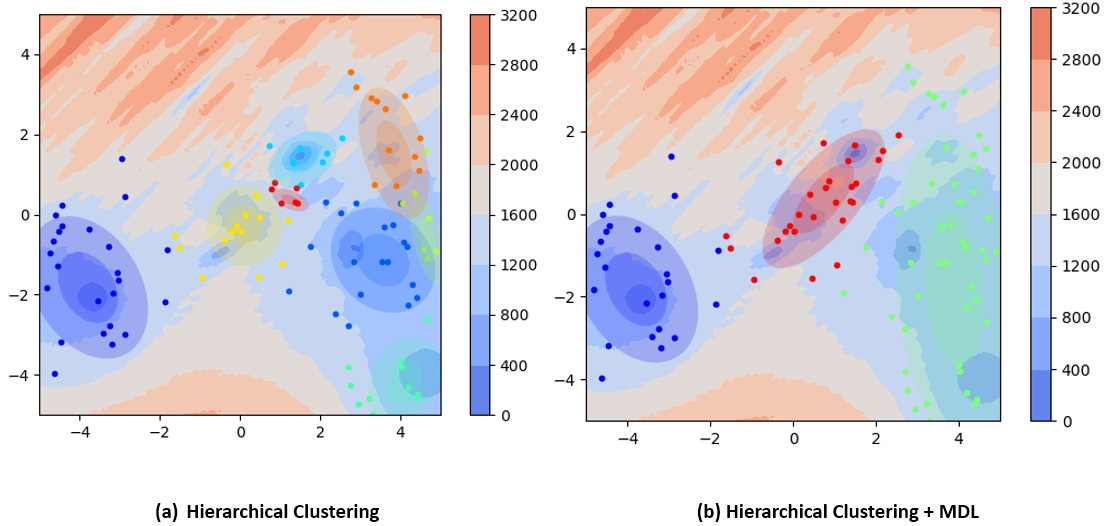
\includegraphics[width=\textwidth]{MDL_comparison_F19}
\caption{Before and after applying Minimal Description Length on CEC2005 F19 Problem}\label{fig:MDL_comparison_F19}
\end{figure}

\begin{figure} 
\centering
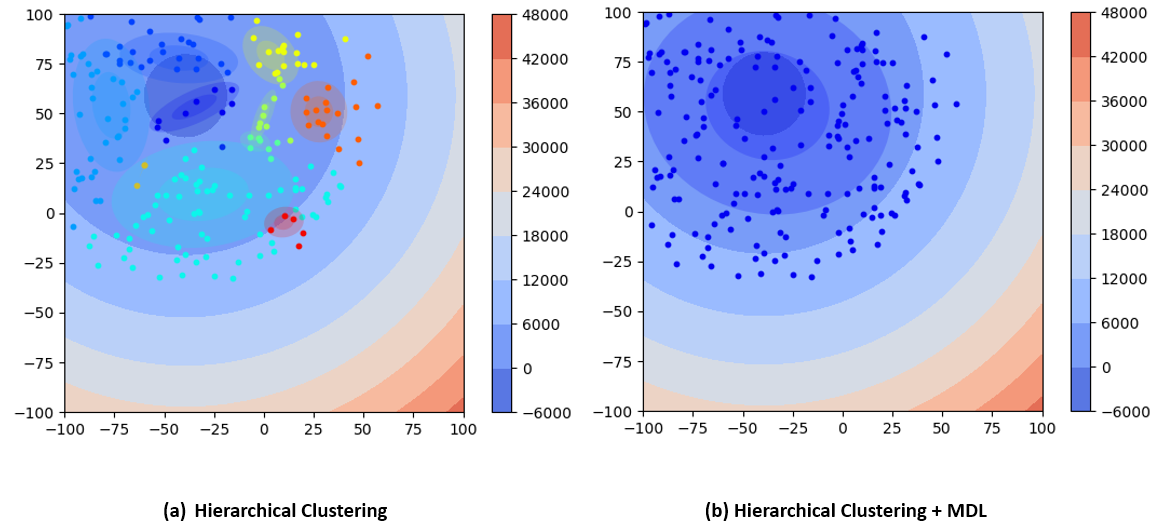
\includegraphics[width=\textwidth]{MDL_comparison}
\caption{Before and after applying Minimal Description Length on CEC2005 F1 Problem}\label{fig:MDL_comparison}
\end{figure}

We can see that for a multimodal problem depicted in Figure~\ref{fig:MDL_comparison_F19}(a), 
the hierarchical clustering technique successfully identifies several fitness hills.
However, for the unimodal problem in Figure~\ref{fig:MDL_comparison}(a), 
the hierarchical clustering creates multiple ``ripples'' on the marginal area.
These clusters are created when the best particle is a bit further from the next best particle.
This indicates that the using the Euclidean distance as the distance metric is not suitable for problems with larger hills.

In order to solve this problem, we assume the underlying hills are composed of multivariate normal distribution.
Given the distribution and a sample position, we can use the \textit{Manhanoblis distance} to serve as a more expressive metric.
We would also like to determine the number of clusters in the beginning, since we believe that the problems are composed of hierarchical hills.
We do not need to invest so much resources in so many regions during the initialization.
Reclustering after a few iterations shall give us a better signal about where to focus.


\section{Minimum Description Length} 
The Minimum Description Length (MDL) principle was introduced by Rissanen in 1978~\cite{Rissanen:1978:MDL}.
It adopts the idea of Occams's razor by selecting the codec that gives the shortest code length of the data.
It provides a natural safeguard against overfitting, 
since it considers not only the goodness of the model, 
but also the complexity of the data to give the hypothesis.
Here we modified the MDL described in~\cite{Kyrgyzov:2007:KMDL} to help us determine the optimum number of clusters that provides the most efficient codes for the sample data.
The MDL considers both \textit{data description accuracy} and \textit{model description efficiency}.


\subsection{Data description accuracy}

Since we would like to take the fitness into account, we use the weighted Gaussian distribution as the underlying model.
For a cluster with $N$ particles, each particle $X_i$ has a rank $r_i$ between $1$ and $N$ (ties are broken randomly) that corresponds to the fitness.
The weight $\omega_i$ can be defined as:
\begin{equation}
\omega_i = \log(N+0.5) - \log(r_i).
\end{equation}

The mean $\mu$ and covariance matrix $\Sigma$ in a weighted Gaussian distribution $N$ can be denoted as:
\begin{equation}
\mu = \frac{1}{\sum_{i=1}^N \omega_i} \sum_{i = 1}^{N} \omega_i X_i,
\end{equation}
\begin{equation}
\Sigma = \frac{1}{\sum_{i=1}^N \omega_i} \sum_{i = 1}^{N} \omega_i (X_i - \mu)^T (X_i - \mu).
\end{equation}


Let $X = \{X_1, X_2, ..., X_I\}$ denote the data set, composed of $I$ samples. 
Each sample is a $D$-dimensional vector $X_i = \{X_{i1}, ..., X_{iD}\}$.  
The class-probability of observing sample $X_i$ in class $j$, described by a parameter set $\Theta_j$, can be denoted as $P_j(X_i|\Theta_j)$.
The probability of observing the sample $X_i$ in a finite mixture model with $J$ components can be denoted as:
\begin{equation}
P(X_i|\Theta) = \sum_{j=1}^J \alpha_j P_j ( X_i | \Theta_j ),
\end{equation}
\begin{equation}
\alpha_j = n_j / I,
\end{equation}
where $\alpha_j$ is the prior probability that $X_i$ belongs to the $j$-th model, 
and $n_j$ denotes the number of samples in cluster $j$.  

Therefore, the probability of observing sample $X_i$ in cluster $j$ can be further described by the $j$-th weighted Gaussain distribution:

\begin{equation}
P(X_i|\Theta_j) = N(X_i | \mu_j, \Sigma_j).
\end{equation}

With the assumption that the data instance $X_i$ are independently distributed, 
the joint data probability is the product of the individual instance probabilities:
\begin{equation}
P(X|\Theta) = \prod_{i=1}^{I} \sum_{j=1}^{J} \alpha_j P_j(X_i | \Theta_j).
\end{equation}

However, we would like to give a higher weight for the data with better fitness.
The weight for $X_{ij}$, the $i$-th particle that belongs to the $j$-th model with rank $r_{ij}$ within the $j$-th cluster, is:
\begin{equation}
\omega_{ij} = \log(n_j+0.5) - \log(r_{ij}),
\end{equation}
and the normalized weight is: 
\begin{equation}
w_{ij} = \frac{\omega_{ij}}{\sum_{i = 1}^{n_j}\omega_{ij}},
\end{equation}
the data description accuracy can be descrived as a weighted sum of individual log-likelihoods:
\begin{equation}
\log(P(X|\Theta)) = \sum_{j=1}^{J}( n_j(\log(\alpha_j) + \sum_{i=1}^{n_j} w_{ij} \log(P_j(X_{ij} | \Theta_j))) ).
\end{equation}


\subsection{Model description efficiency}
Although a more complex model can describe the data distribution better, 
we believe that a simpler model with approximately the same accuracy is better.
Therefore, the number of parameters that a model requires, is also considered in MDL.
The free parameters in the Gaussian mixture model are:
\begin{itemize}
\item $J-1$ paramters for $J$ weights $\alpha_j$, since $\sum \alpha_j = 1$
\item $D$ parameters for each mean $\mu_j$
\item $D(D+1)/2$ parameters for each covariance matrix $\Sigma_j$
\end{itemize}

Therefore, the total number of free parameters is
\begin{equation}
\mathbb{K} = J - 1 + J(D + D(D+1)/2) = J(D^2 + 3D + 2)/2 -1.
\end{equation}


Combining the \textit{data description accuracy} and \textit{model description efficiency}, 
the MDL defined in~\cite{Rissanen:1984:Universal} is denoted as:
\begin{equation}
\min_{\mathbb{K}, \Theta} - \log (P(X|\Theta)) + \frac{1}{2}\mathbb{K}\log(I).
\end{equation}\label{equation:MDL}


\subsection{Model selection with MDL}
As mentioned before, we need to solve the problem of having too many ``ripple'' clusters on the margin area.
Here we would like to use the MDL Equation to calculate model efficiency, and merge overfitting clusters.
Therefore, after identifying potential unimodals with hierarchical clustering in Section~\ref{section:hierarchical},
we use Equation~\ref{equation:MDL} to calculate model efficiency.
We created multiple weighted Gaussian distribution according to the hierarchical clusters, 
as shown in Figure~\ref{fig:MDL_comparison}(a) and~\ref{fig:MDL_comparison_F19}(a).
Then we try all combinations of merging two clusters and calculate the corresponding MDL.
Therefore, we compare the MDL score between the original hierarchical clusters and the new clusters with the minimal MDL score.
If the MDL score of the new model is smaller than the previous model, we repeat the same procedure and keep merging.
This procedure terminates when there is only one cluster remain, or when the minimum MDL score of all possible new modals is larger than the MDL score of the previous model.
Then we get fewer yet still expressive clusters, 
shown in Figure~\ref{fig:MDL_comparison}(b) and~\ref{fig:MDL_comparison_F19}(b).
















\chapter{Linear Projection}
\label{chapter:projection}

We would like to define a region of interest that contains only one uni-model for exploitation.
Also, some algorithms, e.g. SPSO, requires a well-defined hypercube search space with fixed-value constraints in each dimension.
Defining the projection onto subspace can be described as a model selection.
In our case, this process does not require high accuracy, yet has a strict demand on time consumption.
Combining the requirements, we use a linear projection matrix to project the original search space 
onto a subspace with feasible solutions bounded within $[0,1]$ in each dimension.

One of the advantage for using projection matrix is that for a problem with $\ell$ variables, 
a linear projection matrix on homogeneous coordinate only requires $(\ell+1)^2$ hyperparameters to be optimized.
Therefore, less hyperparameters are assigned than directly define each hyperplane borders or vertices.  
This reduces the parameters that we need to optimize and results in less time consumption during model selection.
We also use the (1+1)-Evolutionary Strategy ((1+1)-ES) to optimize the matrix.
The (1+1)-ES is a fast and simple evolutionary strategy,
that allows us to rapidly approximate a high dimensional projection matrix within given number of iterations.

Furthermore, subspace projection also gives advantage for solving \textit{inseparable problems}.
For variabels that are not independent, projection allows the algorithm
to solve an easier, rotated and sheared problem on subspace, as shown in Figure~\ref{fig:Projected_ROI}.
The homogeneous projection matrix seperates the original ROI into less overlapped ROI, 
which reduces redundant search and sometimes enlarges the crutial regions.

In the following sections, we first describe the cannonical affine transformation.
Then we discuss how the projection matrix allows linear projection in a homogeneous coordinate.
Finally, we give details of how we design the cost function and how we utilize the (1+1)-ES to optimize the projection matrix.

\begin{figure}
\centering
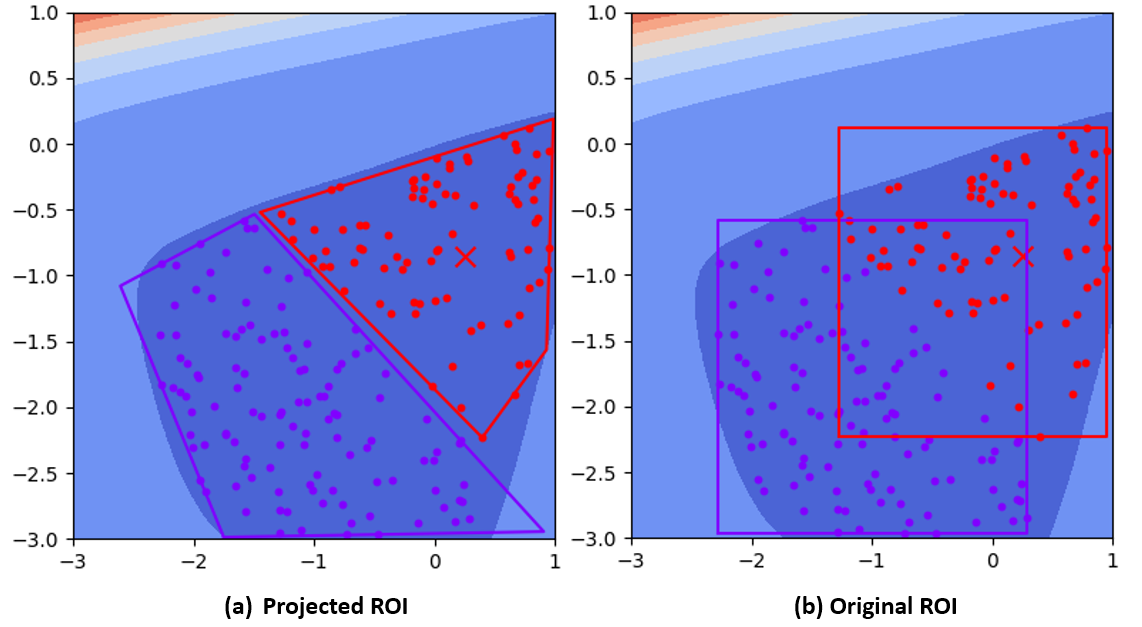
\includegraphics[width=\textwidth]{Projected_ROI}
\caption{Projecting inseparable problems onto subspace.}\label{fig:Projected_ROI}
\end{figure}



\section{Affine Transformation}
In geometry, an affine transformation preserves points, straight lines and planes.
For two affine spaces $A$ and $B$ and any pair of points $P, Q \in A$,
an affine transformation $f$ determines a linear transformation $\varphi$ that can formally defined as:
\begin{displaymath}
\overrightarrow{f(P)f(Q)} = \varphi \overrightarrow{(PQ)}
\end{displaymath}

\subsection{Translation}
\subsection{Rotation}
\subsection{Scaling}
\subsection{Shear}
\subsection{Affine transformation matrix}






\section{Projection}

\subsection{Basic Projection}


\subsection{Homogeneous Coordinate}
Augmented Matrix



\subsection{Perspective Projection}





\section{Optimization for Projection Matrix}

After identifying different clusters of samples, which represents a uni-modal, 
we would like to further define a reasonably good ROI.
In order to obtain a nice ROI for a problem with $D$ variables, 
we need to optimize the $(D+1)^2$ parameters in the projection matrix with a loss function.
The loss function should cost little computational time and should suggest the right direction for optimization, 
in order to match the restrictions of a well-defined ROI.
Also, the optimization only needs to define a reasonably well ROI for the alogirthms to search.  
In the later iterations, the matrix update procedure allows us to define a more accurate ROI with a better insight of the uni-modal subproblem.
In our case, it is acceptable to sacrefice a bit of accuracy for computational time in hyperparameters tuning.  
We will describe the desgin of our loss function and the advantage of using a (1+1)-ES to optimize the matrix in the following sections.  


\subsection{Loss function}

The goal of the ROI is to seperate the search space into non-overlapping subspaces, 
each containing an approximately normalized fitness hill.
Therefore, we would like to keep all the particles that belong to this cluster in the boundary $[0,1]^D$, 
while excluding all the particles that belong to other clusters.
We would also like each underlying model for each subproblem to be a multivariate gaussian distribution with mean around the center $[0.5]^D$
and the covariance matrix to be approximately $0.2I$, where $I$ is an identicle matrix.
Finally, since the we project the particle positions in a homogeneous coordinate, 
the correlations between reconstructed positions on the subspace might not be identicle to the original ones.
We would like to minimize the transformation error.

In our loss function, we considered the following features:
\begin{itemize}
    \item Distances to the boundary for the \textbf{points within the cluster} yet excluded in the ROI.
    \item Distances to the boundary for the \textbf{points of other clusters} yet included in the ROI.
    \item Distance of the weighted \textbf{mean} to the center of subspace $[0.5]^D$
    \item The Mean Absolute Error (MAE) for each element in the weighted \textbf{covariance matrix} to a scaled identicle matrix
    \item The sum of \textbf{reconstruction} error for each particle 
\end{itemize} 

For a possible solution of the projection matrix $X = [x_1, x_2, ..., x_{(d+1)^2}]$ of a problem with $d$ variables, 
we define the loss function $f$ as: 
\begin{equation} 
f(X) = D_should_be_in + D_should_be_out + D_center + MSE_covariance + 
\end{equation}


\subsection{Optimization Algorithms}

Describe the difficulty of finding a fast yet powerful algorithm for \textit{hyperparameters optimization}.

Initialize with a translation + scaling matrix.

We first tried CMA-ES.

Later, we utilize the (1+1)-ES, described in Algorithm~\ref{algo:1+1ES}.



\chapter{Multi-armed Bandit Algorithms}
\label{chapter:MAB}

After identifying the unimodals in Chapter~\ref{chapter:clustering} and defining a ROI for exploitation in Chapter~\ref{chapter:projection},
we still need to decide how to \textbf{allocate our resources}.
During different phases of searching, the \textit{exploration vs. exploitation} dilemma needs to be handled accordingly.
There have been many literatures considering how the algorithms converge 
and how to manipulate the searching step-size in order to find the global optimum more efficiently.
Here, we propose that different strategies should be taken according to \textit{evaluations left}.
Generally, we would like to allow more exploration in the beginning when there are abundant evaluations left.
Then, we would like to gradually increase the portion of exploitation behavior.
When there are very few evaluations left, we should concentrate on exploiting the current best hill.
Therefore, instead of letting the algorithms handle both eploration and exploitation, we propose a bandit technique to help manage the exploration, and leave the simplier subproblems for the alogrithms to exploit.

Multi-armed Bandit (MAB) Algorithms are suitable for this scenario, 
since it learns model from outcomes and the actions it takes do not change the state of the world.
Moreover, the decisions that it makes help discover more knowledge which can improve future decisions.
This matches our description for exploring fitness landscape in real-valued optimization.
However, our goal is a little bit different since we focus more about obtaining the optimum solution.
Unlike canonical MAB algorithms that minimize regrets, we wish to maximize the probability of gaining the maximum rank.

In the following sections, we'll first describe the MAB problem.
Then, we breifly introduce some MAB algorithms 
that were described in the review which Vermorel et. al. made on MAB algorithms~\cite{Vermorel:2005:MAB}.
Finally, we propose a new bandit technique that aims to maximize the probability of gaining the maximum rank.


\section{The Multi-armed Bandit Problem}

Multi-aremed Bandit (MAB) Problem was originally described by Robins in 1985~\cite{Robbins:1985:MAB}.
In this problem, a gambler has to decide which machine and how often to play in a row of slot machines, a.k.a one-armed bandits. 
When played, each machine provides a reward according to a probability distribution.
Therefore, the gambler iteratively plays one lever at each round and observes the probability of reward for each arms.
Here, the gambler is also facing the \textit{exploration vs. exploitation} tradeoff.
The problem of determining the best strategy for the gambler is called the Multi-armed Bandit problem.


The MAB problem can be more formally descirbed as 
an agent deciding which one of the $K \in \mathbb{N}_+$ arms to pull at time $t$ to receive the maximum reward.
The $K$ arms can be seen as a set of real distributions $B = {R_1, ..., R_K}$.
Let $\mu_1, ..., \mu_K$ be the mean of rewards for each arm, and $\mu^* = \max_{k} \{ \mu_k \}$ be the highest reward mean.
The \textit{regret} $\rho$ after $T$ rounds is defined as
\begin{displaymath}
\rho = T\mu^* - \sum_{t=1}^{T} r_t,
\end{displaymath}
where $r_t$ is the reward at time $t$.

The goal is to minimize the regret, which represents the expected difference between the total rewards of an optimal strategy,
and the sum of the actual rewards that have been collected.  
The reason for concerning the regret is because we would like to achieve a \textit{zero-regret strategy}.
A \textit{zero-regret strategy} is a strategy whose average regret per round $\rho / T$ tends to zero with probability $1$ 
when the number of played rounds tends to infinity.
The \textit{zero-regret strategy} are guaranteed to converge to an optimal strategy if enough of rounds are played~\cite{Vermorel:2005:MAB}.



\section{Some common MAB Algorithm}



\subsection{UCB}

\subsection{POKER}
The Price of Knowledge and Estimated Reward (POKER) strategy considers three ideas: pricing uncertainty, exploiting the lever distribution and taking into account the horizon


\section{The New Bandit Technique}



\chapter{The New Multimodal Optimization Technique}
\label{chapter:new_bandit}

In this chapter, we illustrate the proposed multimodal optimization technique step-by-step. 
We first give the framework of the new multimodal optimization technique.
Then we go through details about initialization and unimodal identification.
We also discuss more about the implementation of optimizing projection matrix that defines the ROI.
After that, we explain how to use the proposed multi-armed bandit technique during the optimization.
Finally, we give details about the reclustering criteria, and some of the constraints of our techniques.


\section{Framework of the New Multimodal Optimization Technique}

The goal for our new technique is to identify the potential unimodals in the search space,
define the ROIs for each unimodal for exploitation,
and balance between exploration and exploitation through resource allocation.
First, we need to modify the algorithms to meet some requirements of our technique.
Each algorithm needs to be modified to satisfy the following conditions:
\begin{enumerate}
    \item Able to update one individual at a time 
    \item Able to replace one individual with a given position and fitness
    \item The algorithm can be projected onto a subspace and continue iterating 
\end{enumerate}

Since we consider resource allocation by pulling one arm at a time, 
we need to modify the implementation of algorithms to allow updating one particle at a time.
Also, since we are defining the ROIs by projection, we need the same algorithm to continue after the ROI has changed.
That means, given an updated projection matrix, 
we need to project all the necessary parameters for the algorithms onto to another subspace.
Finally, after clustering, the number samples in one cluster might be more or less than the swarm size required by the algorithm.
Therefore, we need to enable the algorithms to replace particles during optimization.

The new multimodal optimization technique starts with $100D$ samples within the given boundaries of a $D$-dimensional problem.
We use selection pressure 2 to select particles with better fitness to identify potential unimodals in the search space.
We use the hierarchical clustering technique and the MDL method mentioned in Chapter~\ref{chapter:clustering} to determine the clusters.
Then, we define ROIs for each of these clusters with projection matrices, 
which are optimized by (1+1)-ES, as described in Chapter~\ref{chapter:projection}.
After that, we initiate a designated algorithm for each arm on the subspace, initialized with the projected samples in each cluster.
The arms are composed of a projection matrix, which defines the ROI, 
and an algorithm that is modified to allow projection, replacement, and update one particle procedures.
Then we can use the new multi-armed bandit technique to determine resource allocation, i.e. which arm to pull. 
After each iteration, we need to check if the ROI of the latest pulled arm needs to be modified.
We also check if the current cluster is possible to split into smaller clusters, or if any two existing clusters should be merged together.
We'll go through the details of \textit{reclustering} in the following paragraph.
The algorithm terminates if the error reaches a predefined accuracy, or if the number of maximum evaluations is reached.


%The pseudocode of our new algorithm is given in Algorithm~\ref{algo:new_bandit}

%\begin{algorithm}%[t!]
%\caption{Framework of the new Bandit Algorithm}\label{algo:new_banidt}

%$\boldsymbol{X}_{n}$: solution of the $n^{th}$ iteration, $\sigma_n$: step size of the $n^{th}$ iteration, \\
%$N(\boldsymbol{0}, \boldsymbol{I})$: multivariant normal distribution with mean vector $\boldsymbol{0}$ \\ 
%and identical covariance matrix $\boldsymbol{I}$.

%\BlankLine
%\SetKwInOut{Input}{input} \SetKwInOut{Output}{output}
%\Input{ $f$: evaluation function }
%\Output{ $X_{n+1}$: best solution }
%
%\BlankLine
%Initialize $\boldsymbol{X}_0, \sigma_0$ \\
%\While{ termination criterion not met } {
%
%    $\widetilde{\boldsymbol{X}}_n = \boldsymbol{X}_n + \sigma_n N(\boldsymbol{0}, \boldsymbol{I})$  \\
%
%    \eIf{ $f(\widetilde{\boldsymbol{X}}_n) \leq f(\boldsymbol{X}_n) $}{
%        $\boldsymbol{X}_{n+1} = \widetilde{\boldsymbol{X}}_n$ \\
%        $\sigma_{n+1} = 1.5 \sigma_n$
%    }{
%        $\boldsymbol{X}_{n+1} = \boldsymbol{X}_n$ \\
%        $\sigma_{n+1} = 1.5^{-1/4}\sigma_n$
%    }
%}
%
%\Return $\boldsymbol{X}_{n+1}$
%
%\end{algorithm}





\section{Initialization and Unimodal Identification}

In the initialization process, we try to identify the unimodals on the given fitness landscape.
In order to obtain a better resolution, we need a sample size that is large enough, and we need to perform selection after random initilization.
A larger samples size ensures the sampling frequency is high enough to find hills with certain magnitude and width.
We can always discover smaller hills later after the algorithms update the particles.
Yet, it is better to find the right region to search in the first place to reduce unnecessary evaluations.
The selection eliminates some noise for us to further identify the interesting regions.

We start by randomly sample $100D$ points in the given search space of a $D$ dimensional problem. 
Then we select half of the particles with better fitness to get an indication of where the \textit{fitness hills} might be.
After that, we use the selected particles to identify potential unimodals,
using the clustering technique mentioned in Chapter~\ref{chapter:clustering}.
We first perform a hierarchical clustering to consider not only the spatial density, but also the fitness gradients.
It captures the characteristics of the landscape better than K-Means clustering, as explained in Chapter~\ref{chapter:clustering}.
Later we trim down the number of clusters by MDL along with the underlying multivariate Gaussian model.



\section{Define Region of Interest and Construct Arms}

After locating the possible unimodals with the clusters, we can define the ROIs for each cluster 
by projecting the original search space onto a subspace that is only feasible within $[0,1]^D$.
We optimize each projection matrix with the (1+1)-ES and the loss function described in Chapter~\ref{chapter:projection} 
We use the Monte Carlo method to avoid overlapping in higher dimension.
That means, we randomly sample $100D$ points in each subspace $[0,1]^D$ and project them back to the original search space.
Then we project all the sampling points to one particular subspace that needs to be optimized, 
and try to exclude the samples from other clusters out of the feasible region $[0,1]^D$
The projection matrices are optimized one-by-one, so the order might effect the optimization results.
However, the initial clustering techniques provide a cluster approximate to a multivariate Gaussian distribution.
Therefore, the clusters are more likely to be in a ``round'' shape, that can be easily fit into a quadrilateral.  


With the optimized ROIs and the samples in each clusters, 
we can initiate the arms for the new multi-armed bandit technique mentioned in Chapter~\ref{chapter:MAB}
Each arm is composed of a \textbf{projection matrix}, that defines the ROI on the original search space,
the mean $\mu$ and covariance matrix $\Sigma$ of the underlying Gaussian model,
and a \textbf{designated algorithm} with population size $n$, that performs optimization on the subspace.
Notice that whenever an evaluation is needed for the algorithm, we project the position on the subspace back to the original space for evaluation.
Therefore, the algorithm always conduct on the subspace without knowing the original search space.
In order to initiate the algorithm, we need to modify the number of particles in each cluster to meet the required population.
For clusters with samples more than $n$, we select the top-n particles with the best fitness.
For clusters with samples less than $n$, we sample uniformly random points on the $[0,1]^D$ subspace and inverse project it with the projection matrix back to the original search space to evaluate their fitness.
Then we add them into the clusters and initiate the algorithm on the subspace.


\section{Remain Evaluations Allocation and Recluster}

In order to determine which arm to pull, we need to calculate the best remain evaluation allocation, as described in Chapter~\ref{chapter:MAB}.
We normalize the allocation vector and add it to a $k$-length record vector, where $k$ is the total number of arms/clusters.  
During each iteration, we select the best arm, i.e. the arm that gives the highest value in the record, to update.
We than minus the record value of that arm with 1, and ask the algorithm of the best arm to update one particle.
Then we recalculate the remain evaluation allocation and add it into the record again.
This way, the number of times each arm has been pulled should be asymptotically close to the time-variant resource allocation.

Right after each update, we check whether if we need to update the projection matrix to place the best point at the center of the ROI.
This is done by a statistic test, which compares the weighted mean of the new samples against the original underlying multivariate normal model.
Given a set of samples $X_1, ..., X_n \sim N_{D}(\mu, \Sigma)$ coming from a $D$-dimensional normal distribution with $\mu$ and $\Sigma$ known. 
For testing $H_0: \mu = \mu_0$ versus $H_1: \mu \neq \mu_0$, the statistic
\begin{displaymath}
Z = ( \bar{X} - \mu_0 )^T (\frac{\Sigma}{n})^{-1} ( \bar{X} - \mu_0 ) = n( \bar{X} - \mu_0 )^T \Sigma^{-1} ( \bar{X} - \mu_0 )
\end{displaymath}
is used that follows $ \chi^{2}(D)$-distribution under $H_0$.
This is a generalization of the $z$-test, also known as $u$-test.
We use this statistic test to examine if the new samples still comes from the same underlying multivariate normal distribution the ROI is constructed on.
If the new samples is rejected by the statistic test that they do not come from the underlying distribution, 
we update the projection matrix of this specific arm to reallocate the ROI.

Whenever the ROI is updated, we also check if number of clusters should alter.
This process is called \textit{recluster}.
We first need to check if the cluster in the current best arm can be split into multiple clusters 
with the hierarchical clustering and MDL techniques described in~\ref{chapter:clustering}.  
Then, we check if any two clusters in the search space can be merged together 
using simply the MDL method mentioned in Chapter~\ref{chapter:clustering}.  
This is a stable way to avoid ``cracking'' at the borders of different clusters.
Also, whenever the recluster occurs, we reinitialize the record vector, since the clusters might be different from the last setup.



\chapter{Experiments}
\label{chapter:experiments}

We use 25 benchmark problems from the CEC 2005 Special Session on Real-Parameter Optimization to test the performance of our new techniques.
The CEC 2005 benchmark problems are composed of both standard test problems \textit{e.g.} Sphere, Schwefel's, Rosenbrock's, Rastrigin's, etc.,
and some hybrid problems.
We tested the CMA-ES, PSO, and ACO$_R$ algorithms with and without our new techniques.
The results show that our technique reduces the average error of CMA-ES and ACO$_R$ on some multimodal problems.  

\section{CEC 2005 Benchmark Problems}

The special session on real-paramter optimization of CEC 2005~\cite{Suganthan:2005:benchmark} aims to evaluate different algorithms in a more systematic manner by specifying a common termination criterion, size of problems, linkages/rotation, etc.
It consists of 25 minimization problems with $2, 10, 30, 50$ dimensions.
The evaluation requires 25 runs, each with maximum evaluations $10000 * D$. 
Initialization is required to be uniform random within the search space, except for problems 7 and 25, for which initialization ranges are specified.
Similarly, the global optimum exists within the given bounds, except for problem 7 and 25.
The algorithm is terminated one it reaches the maximum evaluations or if the minimum error in the function value is less than $10^{-8}$.
Here we only tested on the 2-dimensional problems, 
since our technique consumes too much time on higher dimensions, 
making optimization impractical.  
Also, we modified the Problem 11 and 12 by adding the Euclidean distance to the bias position in the fitness function,
so that there exists only one global optimum solution in the search space.
Further speedup and studies to expend the technique on higher dimension are needed.
We show the average and median error plots for all 25 problems in the following section.
%The tables, following the requested format in~\cite{Suganthan:2005:benchmark}, are also given the the following section.  


\section{Experiment Settings}

In this section, we briefly describe the parameters setting for CMA-ES, SPSO and ACOR.

We use the \textit{Covariance Matrix Adaptation Evolution Strategy for non-linear numerical optimization in Python} package~\footnote{https://pypi.python.org/pypi/cma} provided by Hensen, the author of CMA-ES.
Although the default population for CMA-ES in $D$-dimension is set to be $4 + \lfloor3\log(D)\rfloor$, meaning default population size is 6 in 2D,
we found out that we a larger population for the MDL to not merge every particles into one cluster.
Therefore, we set the population size as 30 for CMA-ES.
The initial mean is set to be the center between max bounds and min bounds in every dimension.
The initial step-size is set to be one sixth of the maximum length between max bounds and min bounds in each dimension. 
It is suggested to let the global optimum be within three standard deviation~\cite{Hansen:2006:CMA_ES_review}.

As for the SPSO 2011, there are currently no official Python implementation, 
so we created our own Python implementation according to the tutorials~\cite{Clerc:2012:SPSO2011},
and the official SPSO 2011 C++ code provided by Clerc, the author of SPSO~\footnote{https://www.particleswarm.info}.
The population size is set to be 40 as suggested in~\cite{Clerc:2012:SPSO2011}.
The parameters $c = \frac{1}{2} + \ln(2) \simeq 1.193$ and $w = \frac{1}{2\ln(2)} \simeq 0.721$ are also set as default.
We implement the random topology with $K = 3$,
and update the topology at the beginning and in every iteration when the best fitness does not improve.
Also, we use the ``bounce back'' boundary condition suggested in~\cite{Clerc:2012:SPSO2011}, which is also described in Chapter~\ref{chapter:algos}.

For ACOR, we set our parameters according to the original paper~\cite{Socha:2008:ACOR}. 
The parameters are shown in Table~\ref{table:ACOR_parameters}.

\begin{table}%[t!]
\centering
\label{table:ACOR_parameters}
\begin{tabular}{lll}
\hline
Parameter                        & Symbol   & Value          \\ \hline
No. of ants used in an iteration & $m$      & $2$            \\
Speed of convergence             & $\xi$    & $0.85$         \\
Locality of the search process   & $q$      & $10^{-4}$      \\
Archive size                     & $k$      & $50$           \\ \hline
\end{tabular}
\caption{Summary of the parameters used by $ACO_R$}
\end{table}

%Describe our bandit parameters setting, including the initial population, maximum number of arms, and (1+1)-ES step size.

\section{Experiment Results}

Generally speaking, we can see a huge improvement in multimodal problems and hybrid problems
when combining our technique with ACO$_R$,
since the underlying model for ACO$_R$ is a Gaussian Kernel that intrinsically models hills.
We can see improvement in some cases when combining our technique with CMA-ES.
However, for SPSO, most of the results costs more evaluations to get to same error level.
This is because the underlying model for SPSO is not a Gaussian, but a random topology.
The flying particles make reclustering and redefining ROIs really unstable.


Problems 1 to 5 are unimodal functions.
The optimum solution of Problem 5 is on the diagonal of the search space, 
making it extremely easy to solve for SPSO and ACO$_R$.
Thus there is no error line for these two algorithms on Problem 5
We can see that CMA-ES is extremely efficient on solving unimodal problems, 
since the underlying model is a multivariate Gaussian and it converges very fast.
As expected, our methods to cost slightly more evaluations than the original algorithms on unimodal functions,
since we sample more points in the beginning. 
Also, although our clustering methods recognize unimodals in most of the times,
it is not good at handling narrow valleys, \textit{e.g.} Problem 3, 
and starts to split into multiple clusters once falls into the valley with small gradient.
This multiplication gets worse since the smaller the ROI becomes, the less gradient info there is.
Thus, the clustering methods would try its best to generate ``hills'' from the plane with almost no gradient.
This is the reason why our technique does not improve the original algorithms.
it falls into the valley


Problems 6 to 12 are basic multimodal functions.
We can see significant improvement in Problem 11 and Problem 12 on algorithm CMA-ES and ACO$_R$.
Besides, ACO$_R$ combined with our techniques leads with the minimum error in most of the problems.
This means that the divide-and-conquer technique works well on problems with multiple hills.
The narrow valley characteristics also appears in Problem 6, so we spend more evaluations than the original algorithms.
One interesting thing happens in Problem 9, where our technique failed to improve CMA-ES on a Rastrigin Problem.
We suspect that it is due not being able to recognize the small hills, since CMA-ES samples with a normal distribution.
Therefore, even if particles did get to the top of different hills, the MDL method would still recognize them as one normal distribution.
Thus, no reclustering was performed and the population converged to the wrong hills sometimes.

Problem 13 and Problem 14 are expended problems, and they are a bit too difficult for most of the algorithms.

Problems 15 to 25 are hybrid composition functions.
SPSO is suitable for these kinds of problems, since SPSO is good at exploring and takes a bit longer to converge.
However, our methods enhanced the ability of ACO$_R$, making it compatible with SPSO, and even better sometimes.



\begin{figure}
\centering
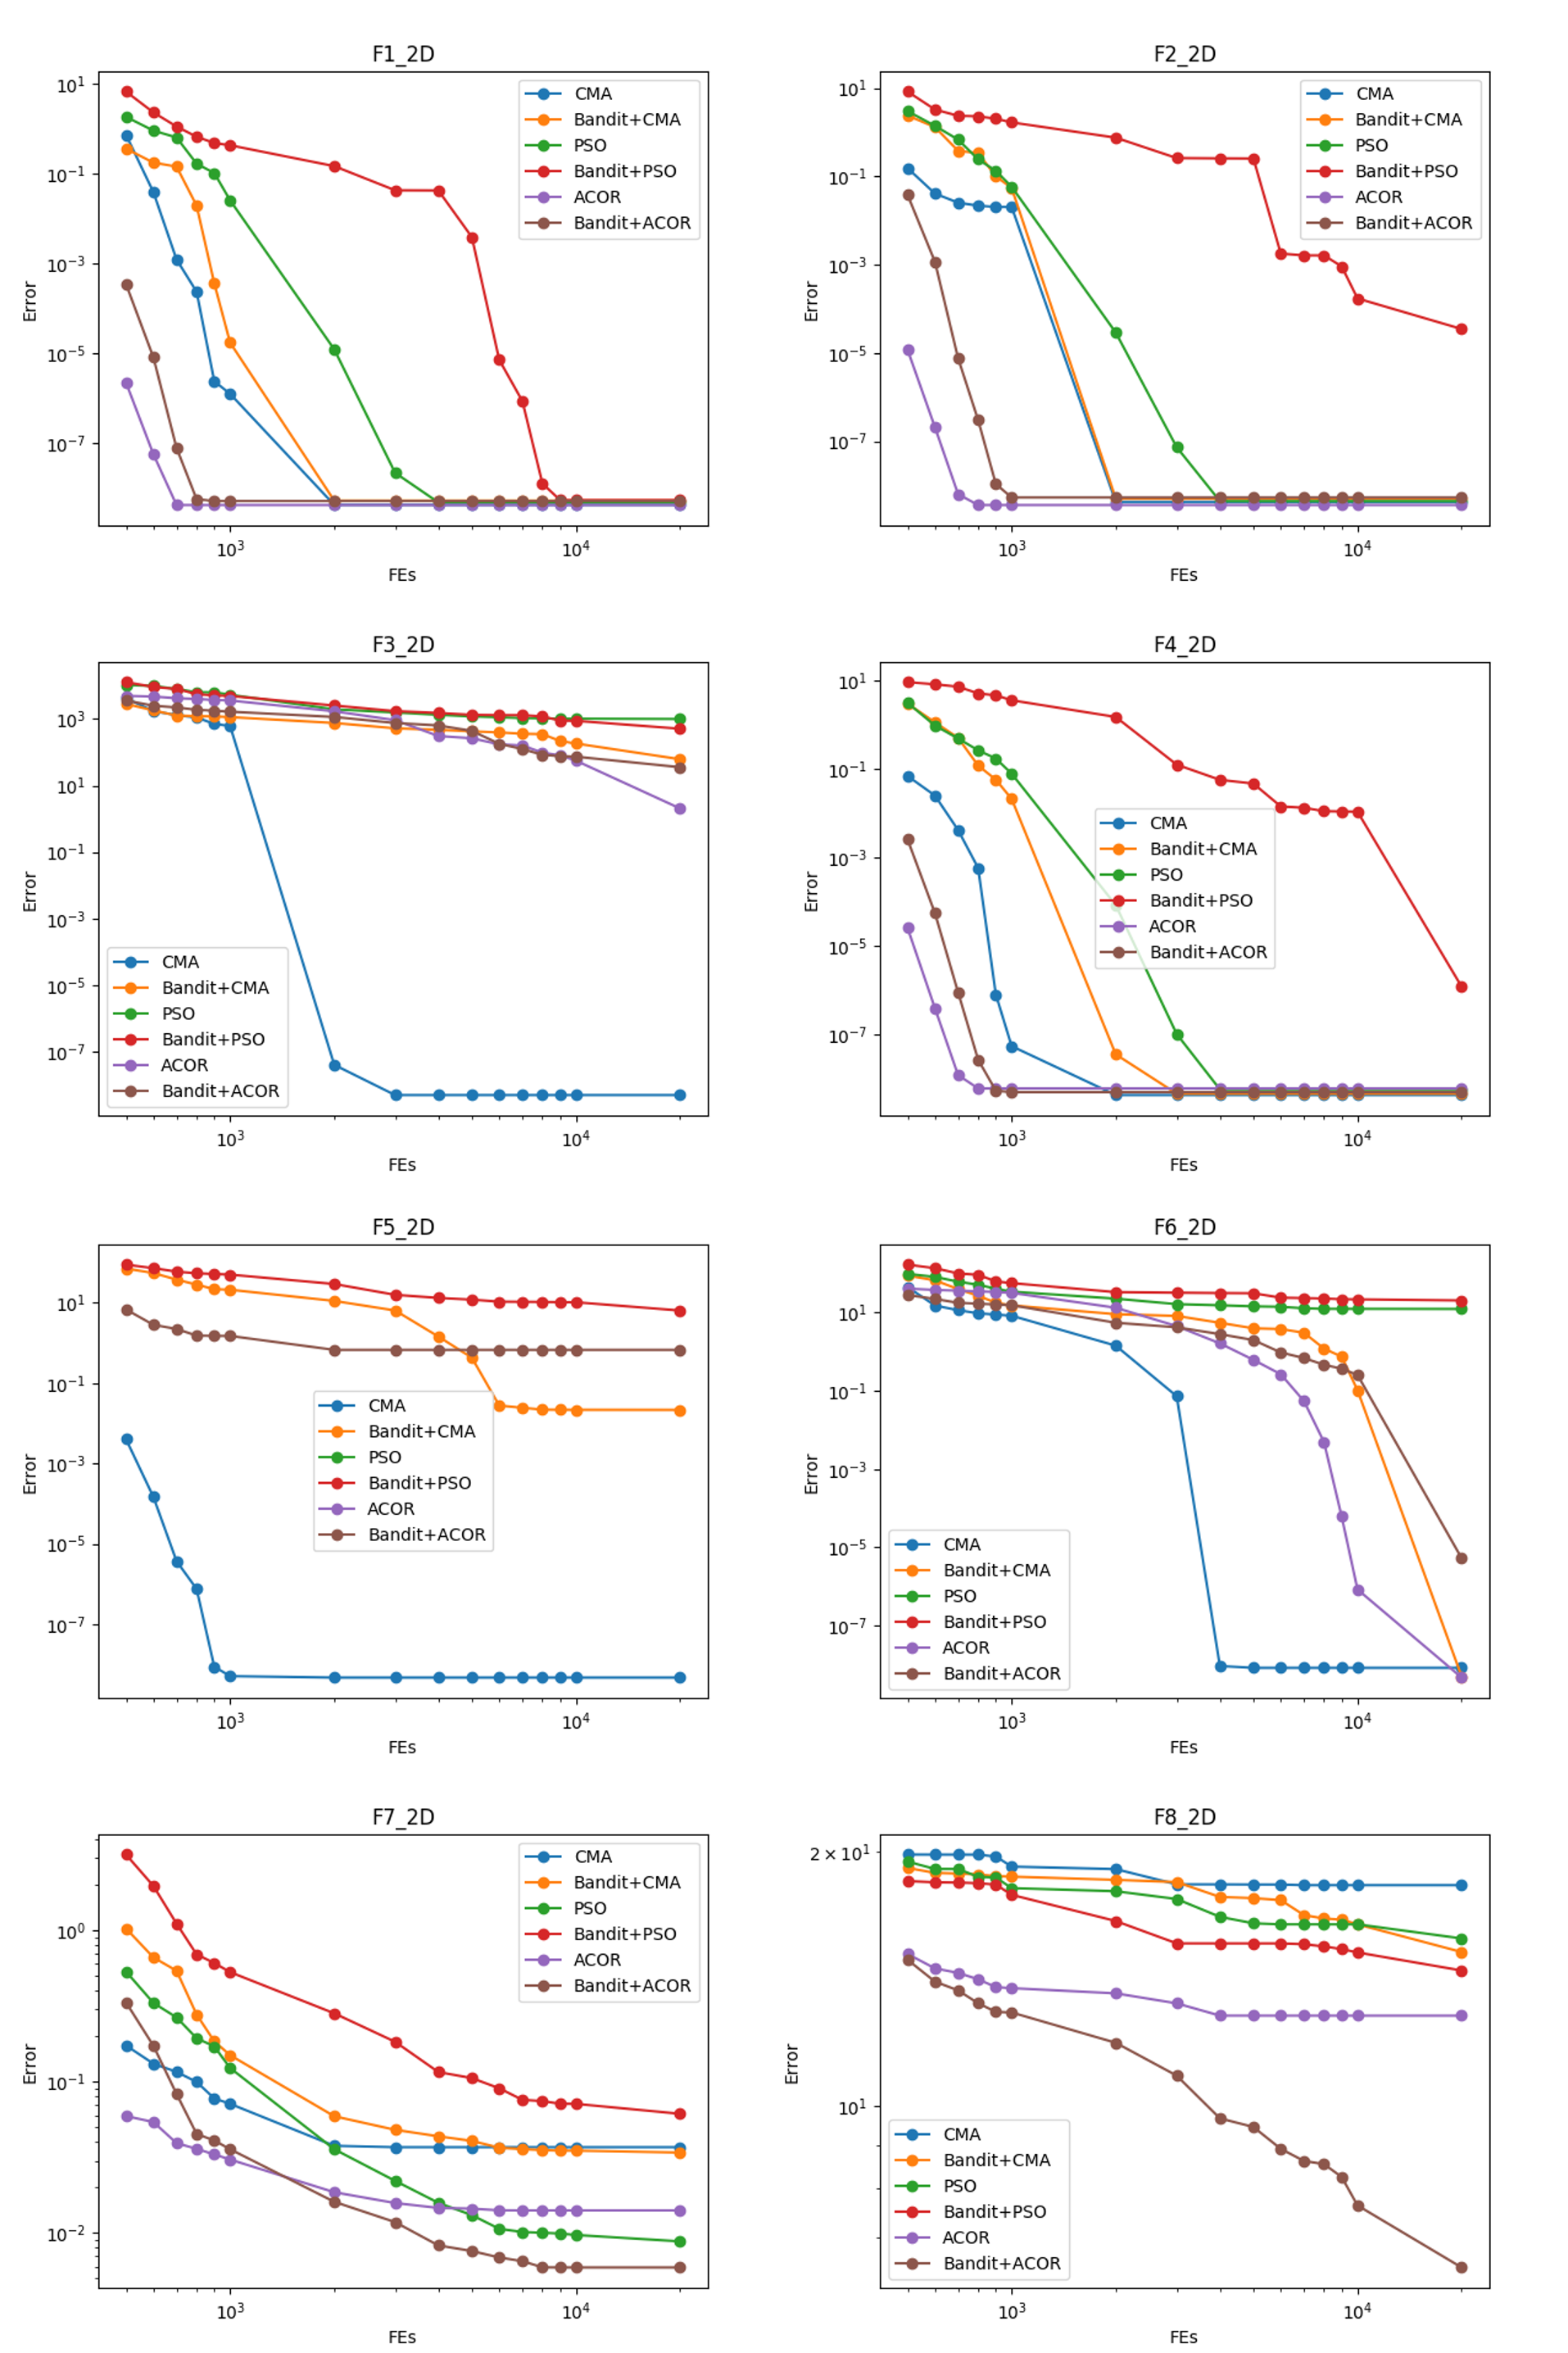
\includegraphics[width=\textwidth]{Average_F1_F8}
\caption{Average error of Problem 1 to Problem 8.}\label{fig:Average_F1_F8}
\end{figure}

\begin{figure}
\centering
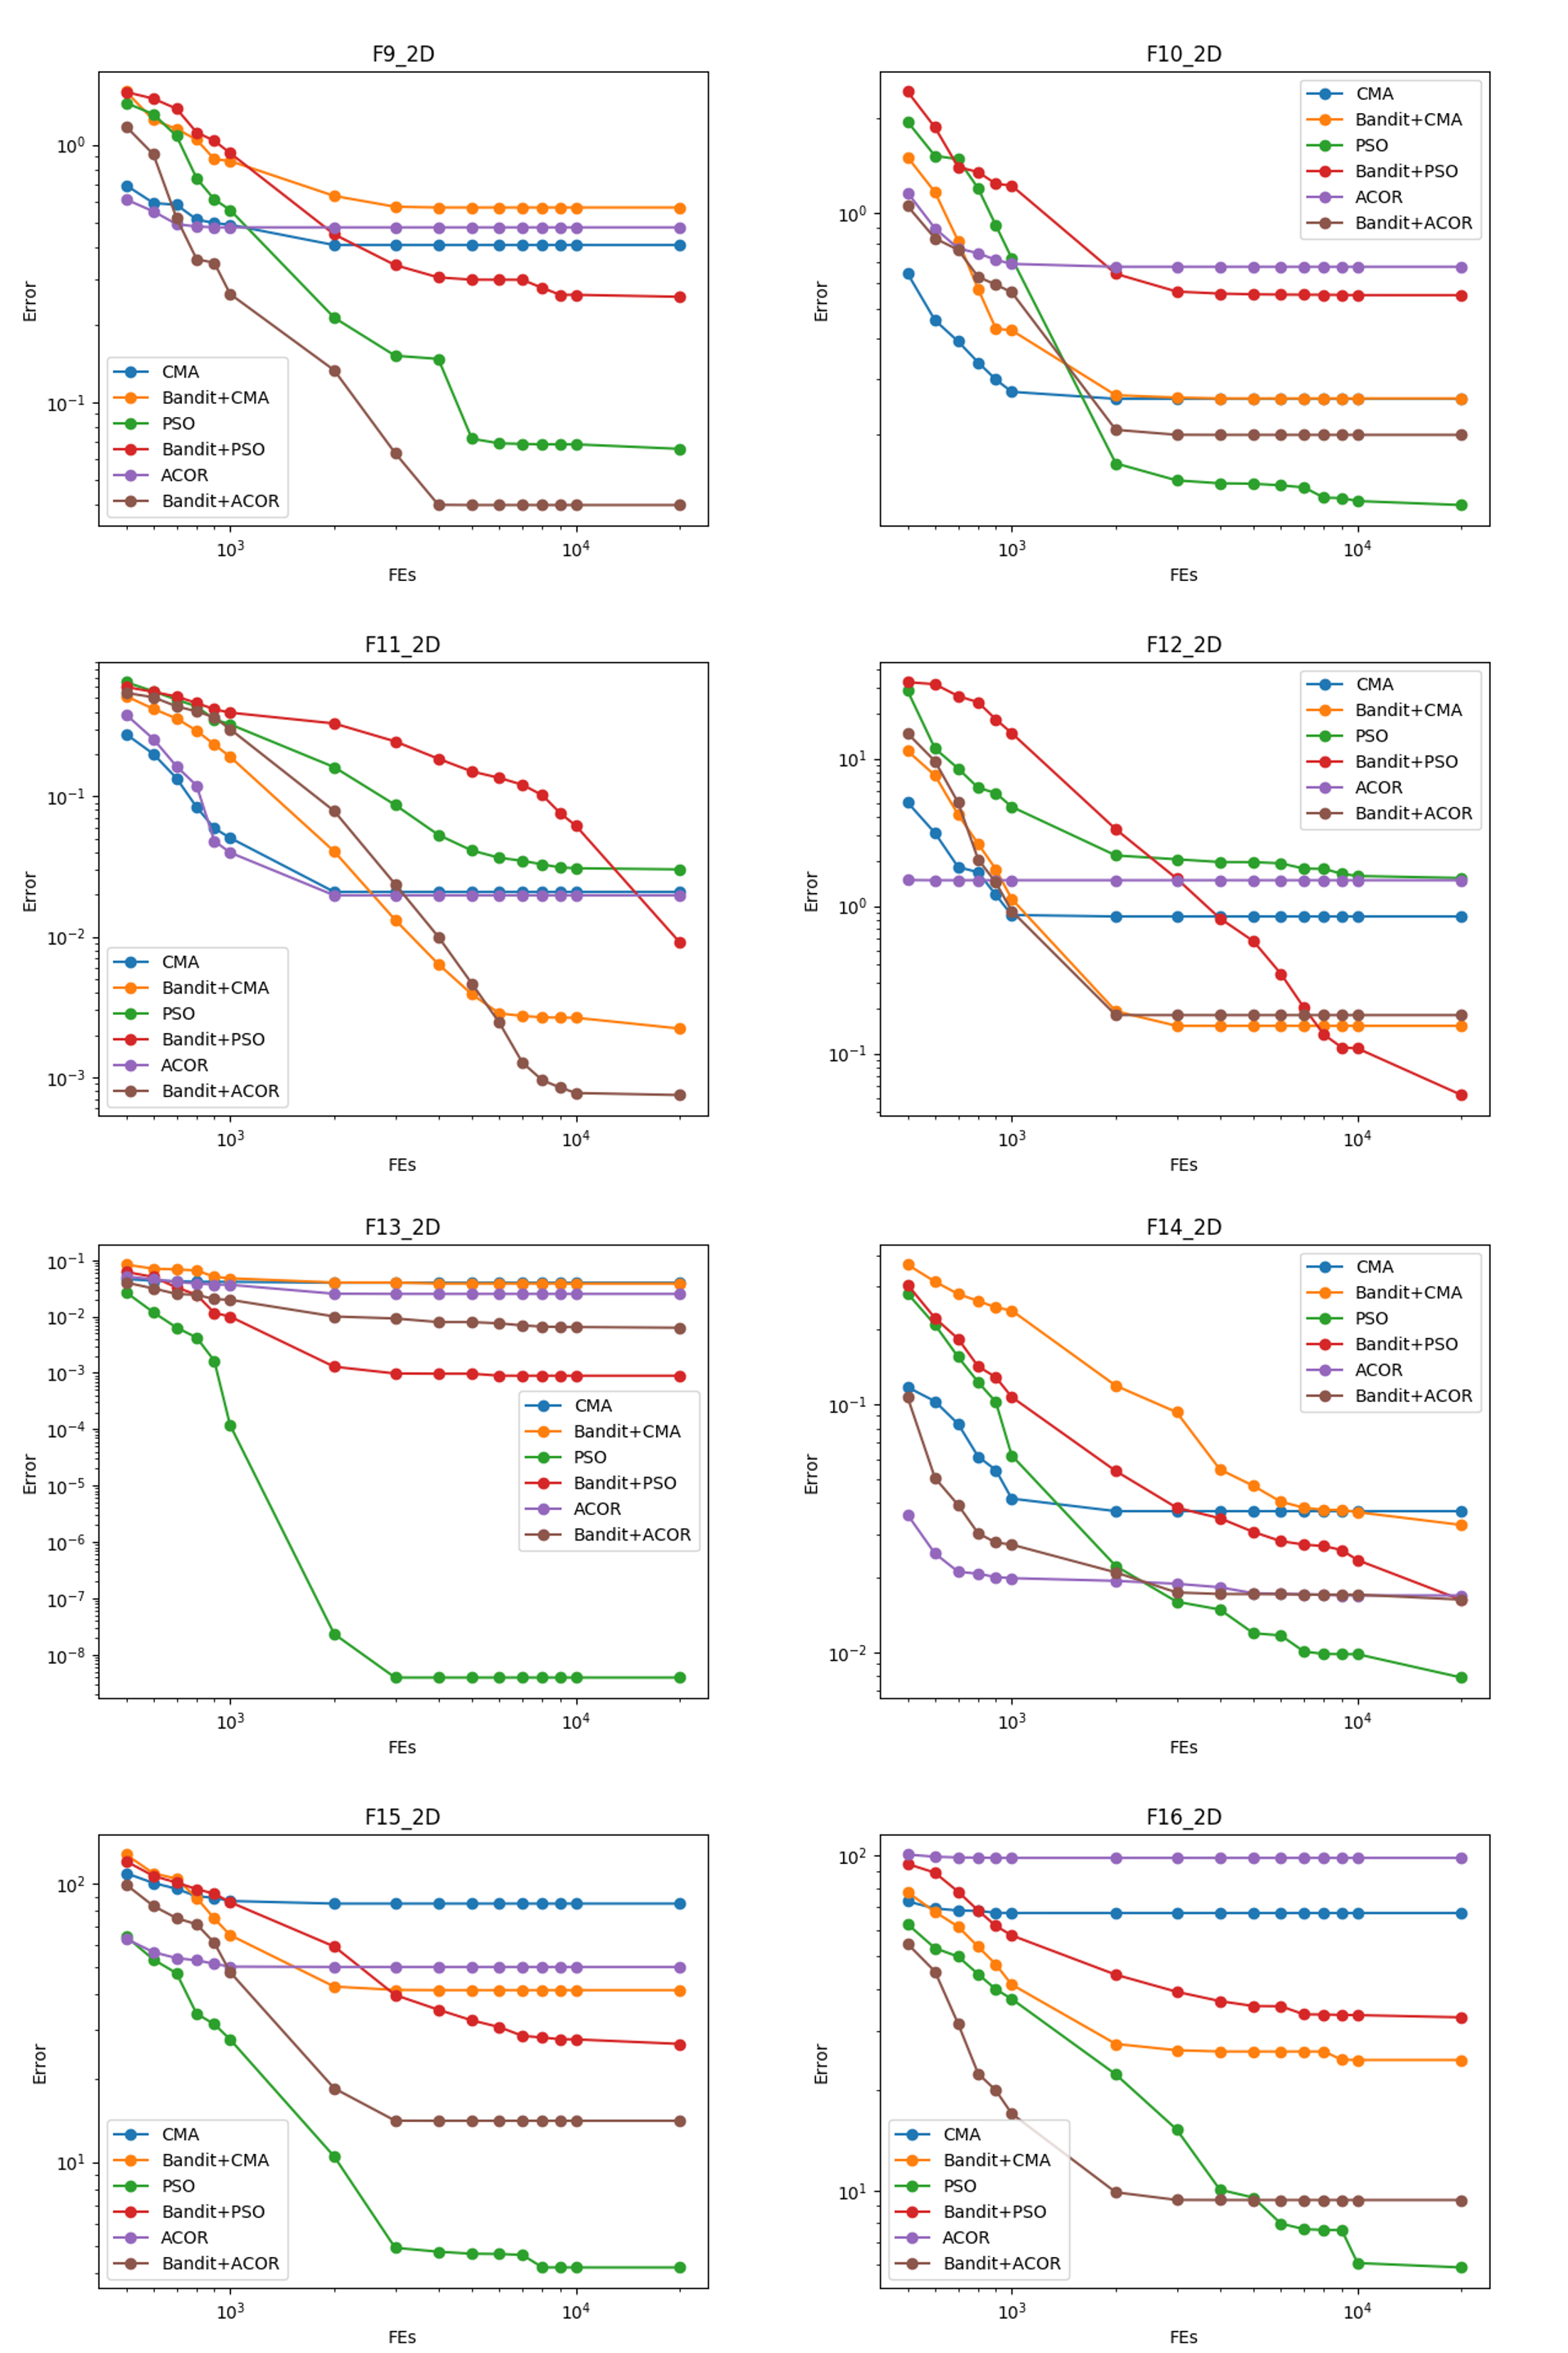
\includegraphics[width=\textwidth]{Average_F9_F16}
\caption{Average error of Problem 9 to Problem 16.}\label{fig:Average_F9_F16}
\end{figure}

\begin{figure}
\centering
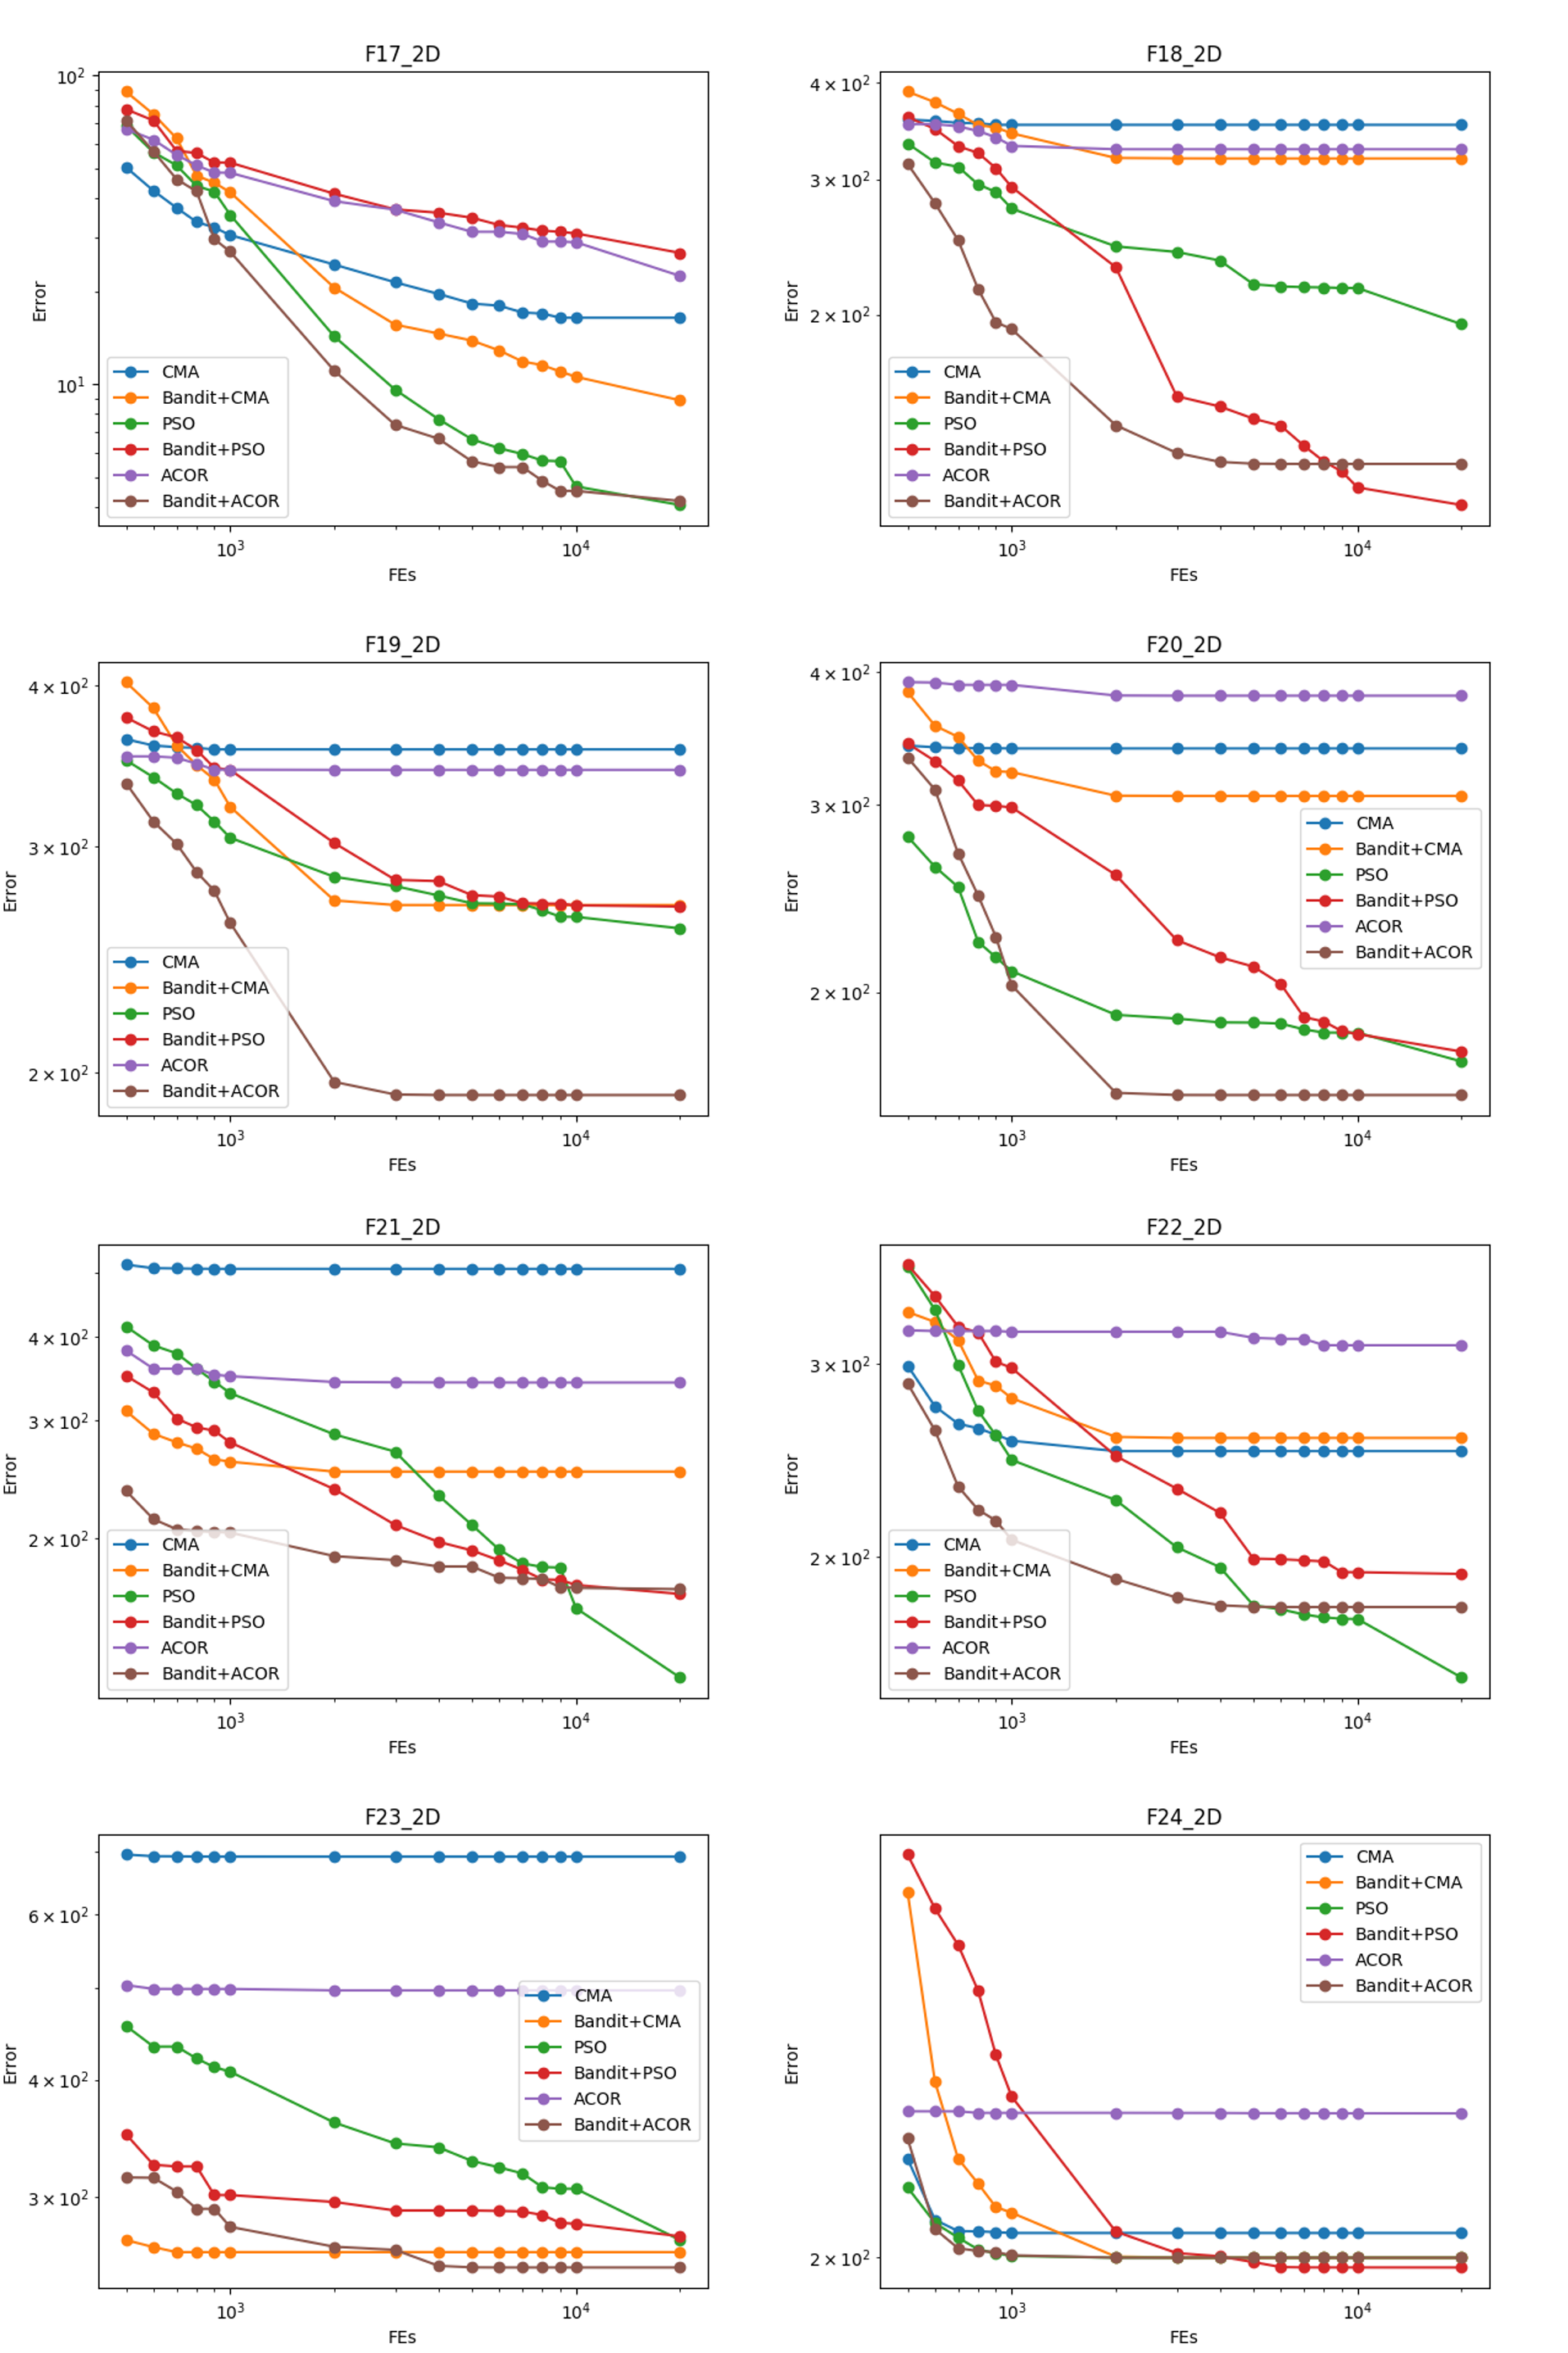
\includegraphics[width=\textwidth]{Average_F17_F24}
\caption{Average error of Problem 17 to Problem 24.}\label{fig:Average_F17_F24}
\end{figure}

\begin{figure}
\centering
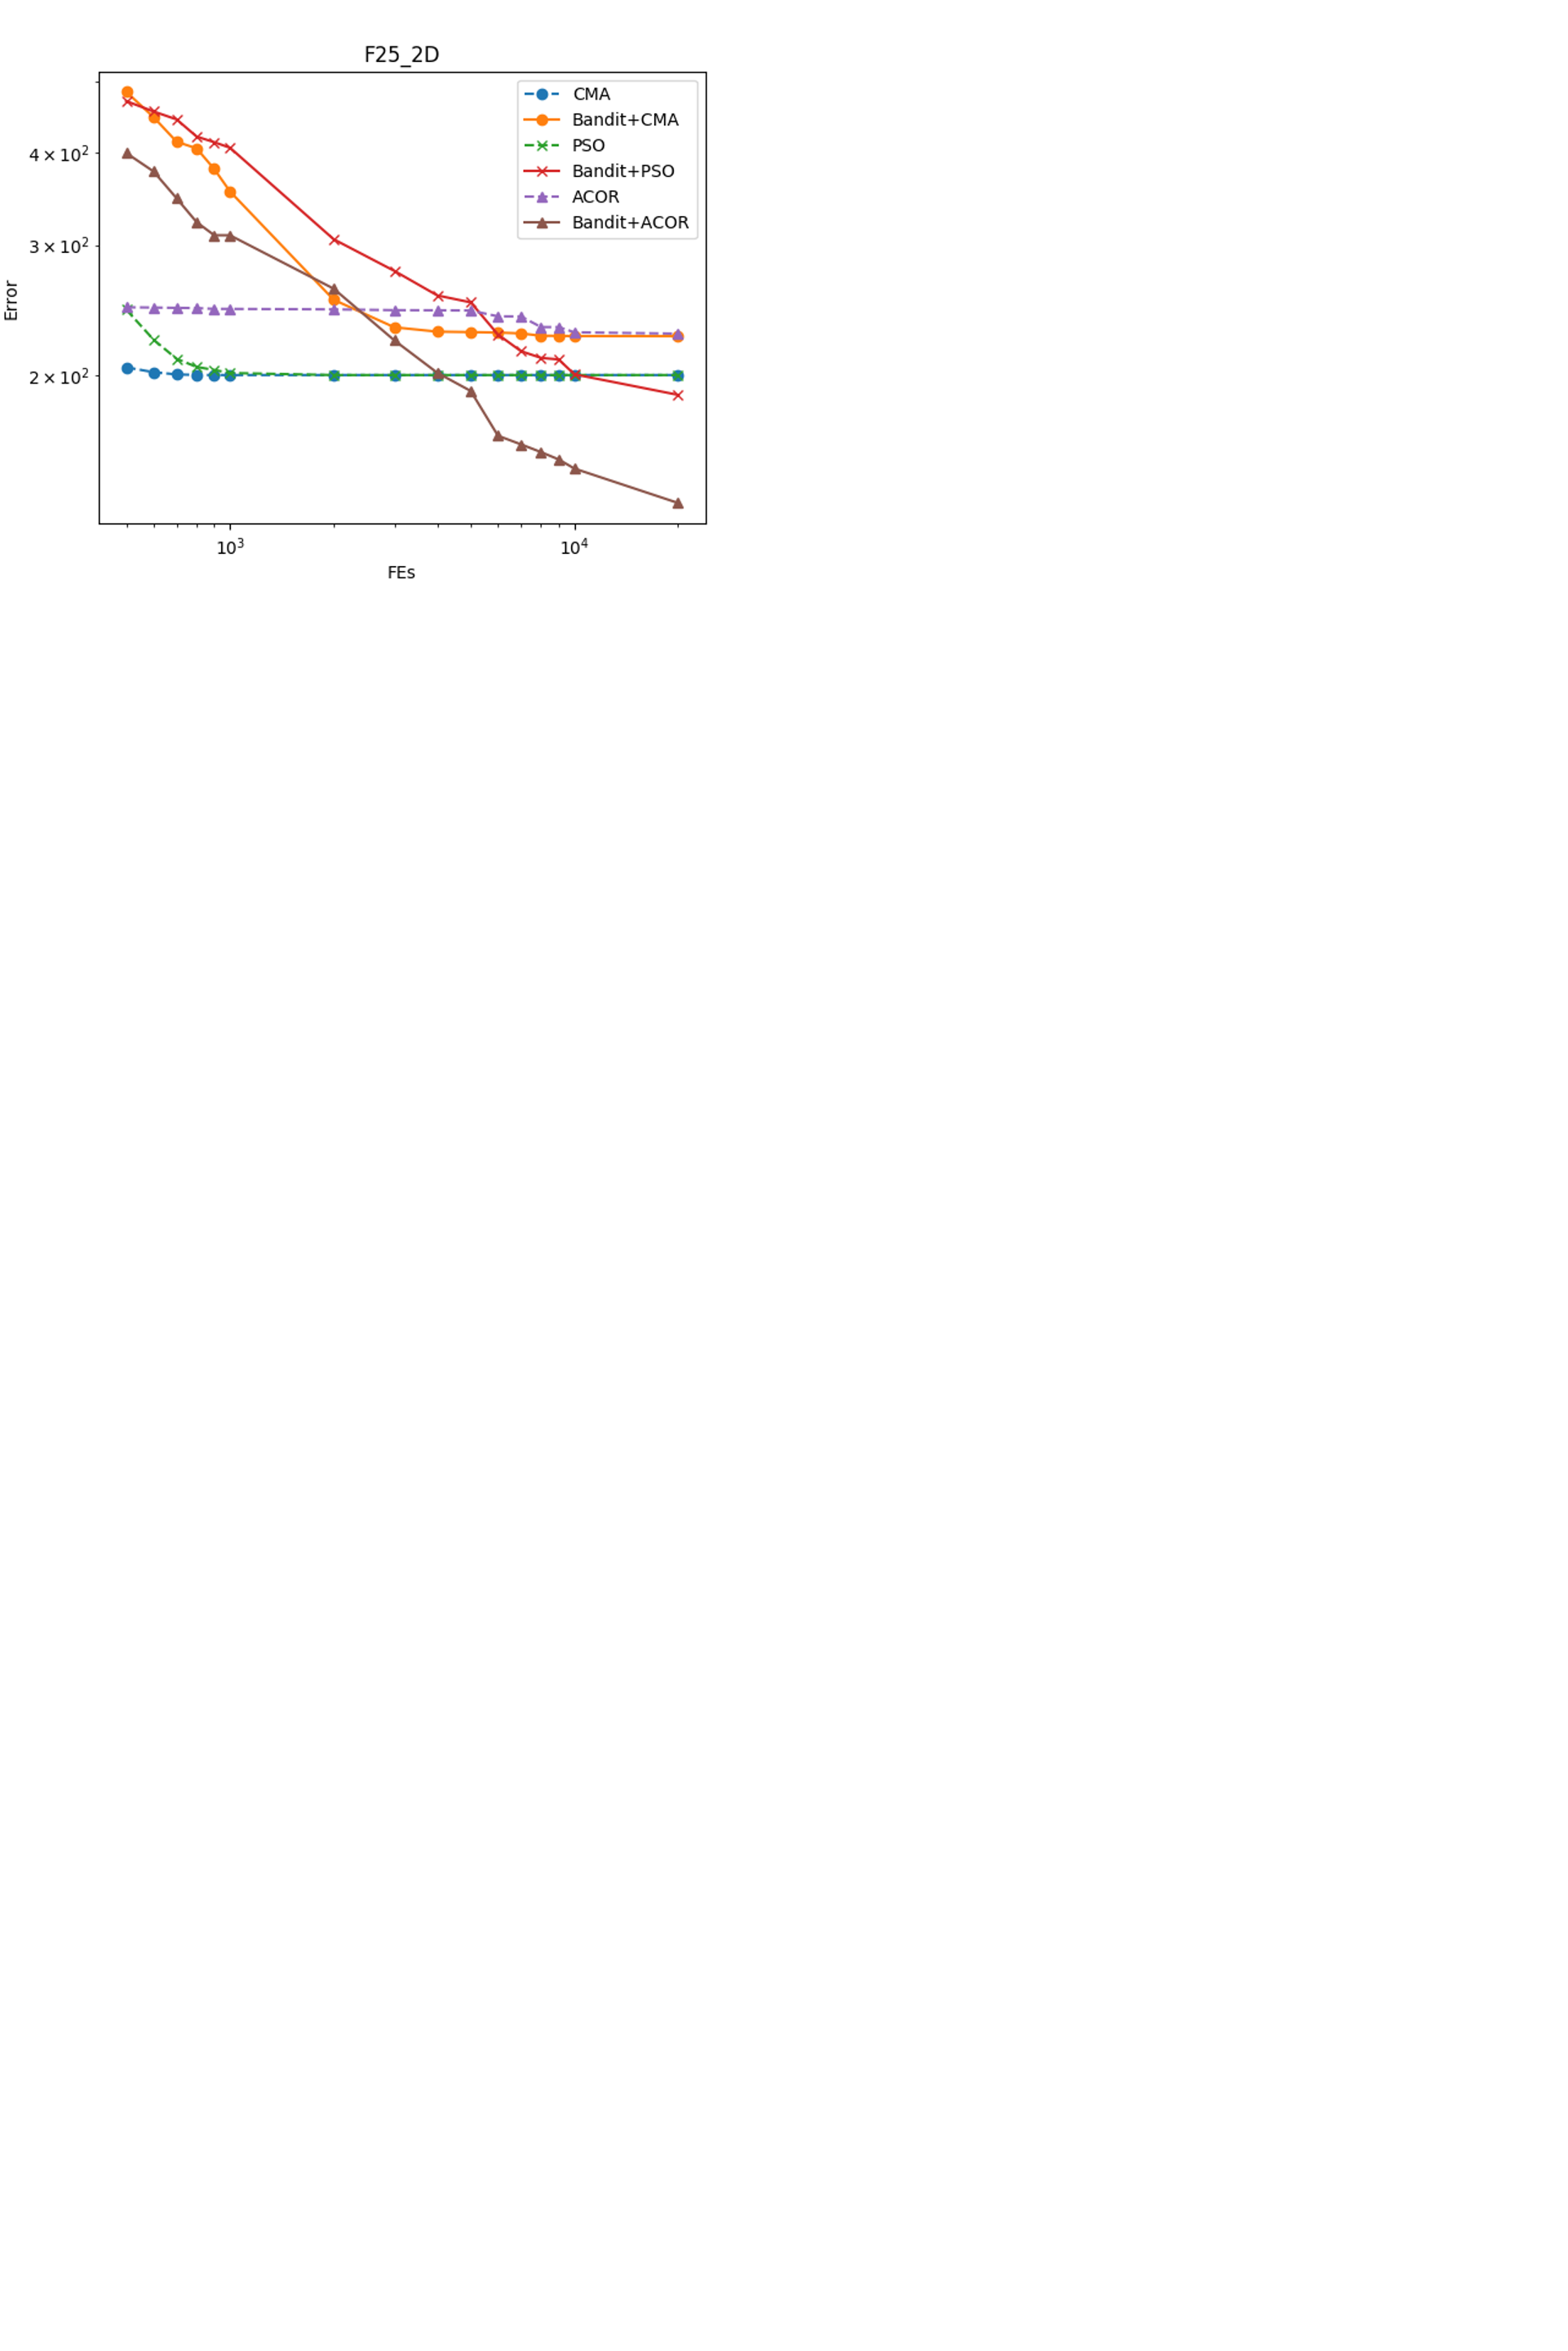
\includegraphics[width=\textwidth]{Average_F25}
\caption{Average error of Problem 25.}\label{fig:Average_F25}
\end{figure}

\begin{figure}
\centering
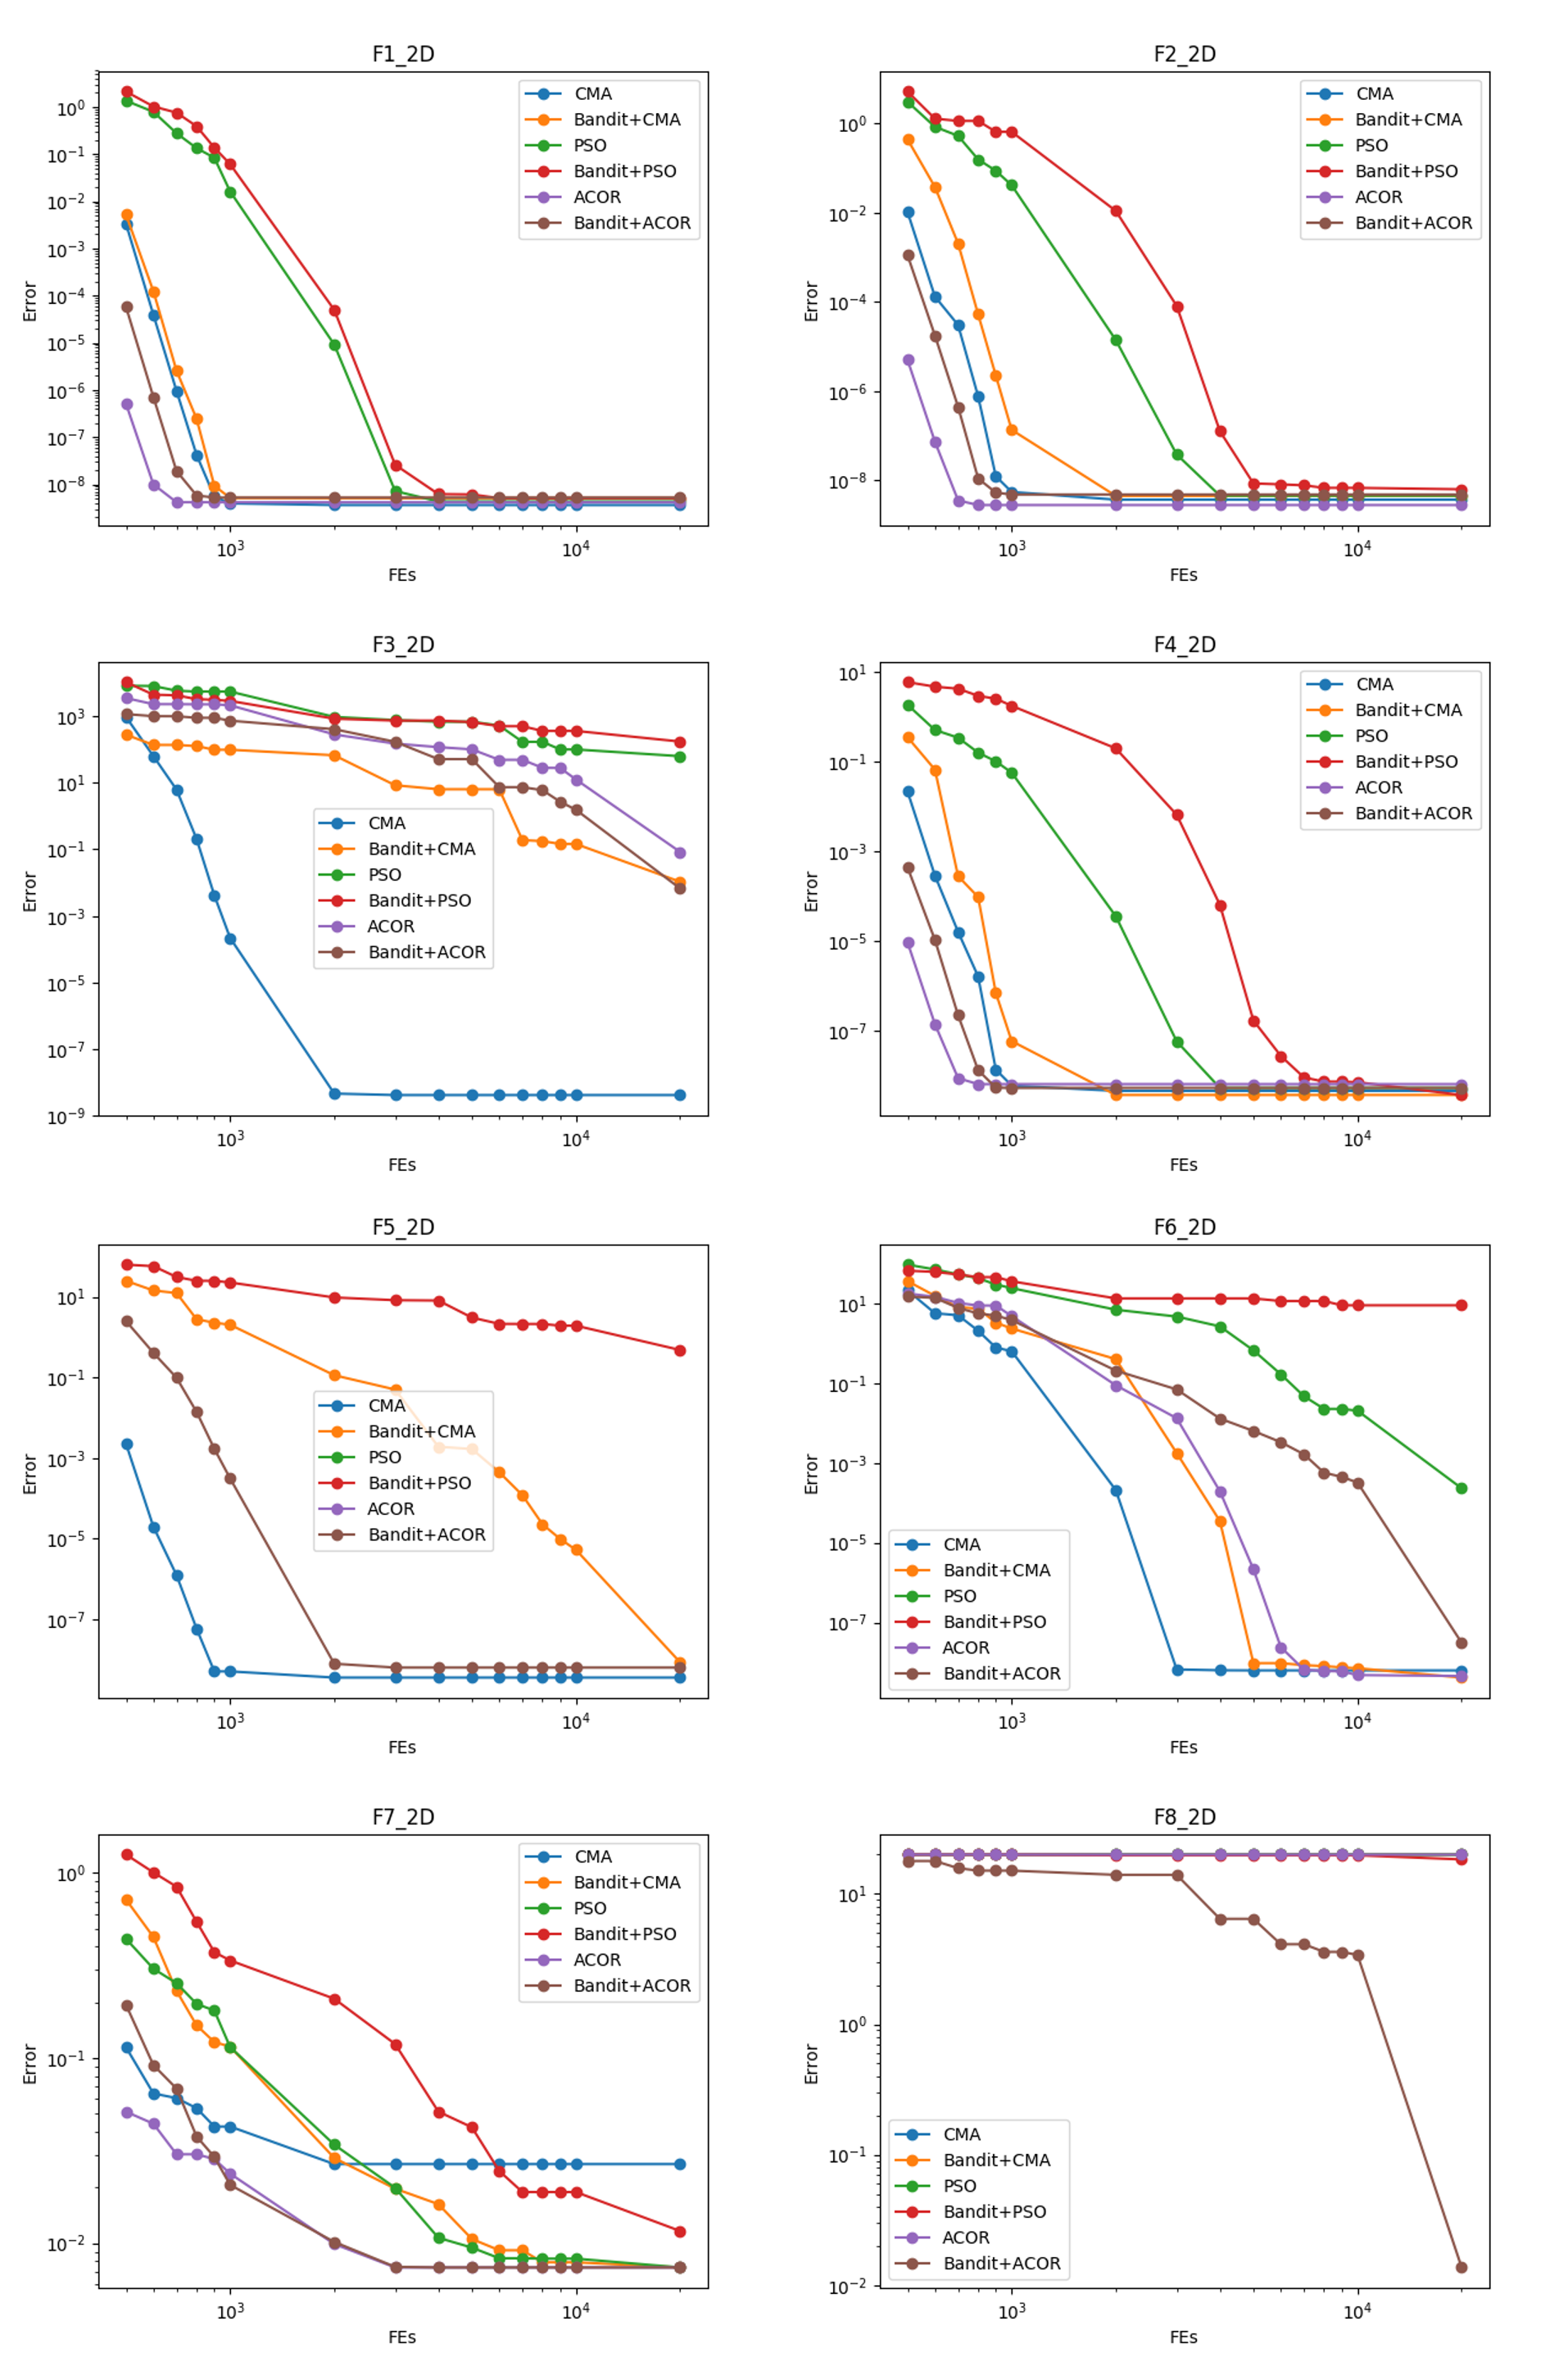
\includegraphics[width=\textwidth]{Median_F1_F8}
\caption{Median error of Problem 1 to Problem 8.}\label{fig:Median_F1_F8}
\end{figure}

\begin{figure}
\centering
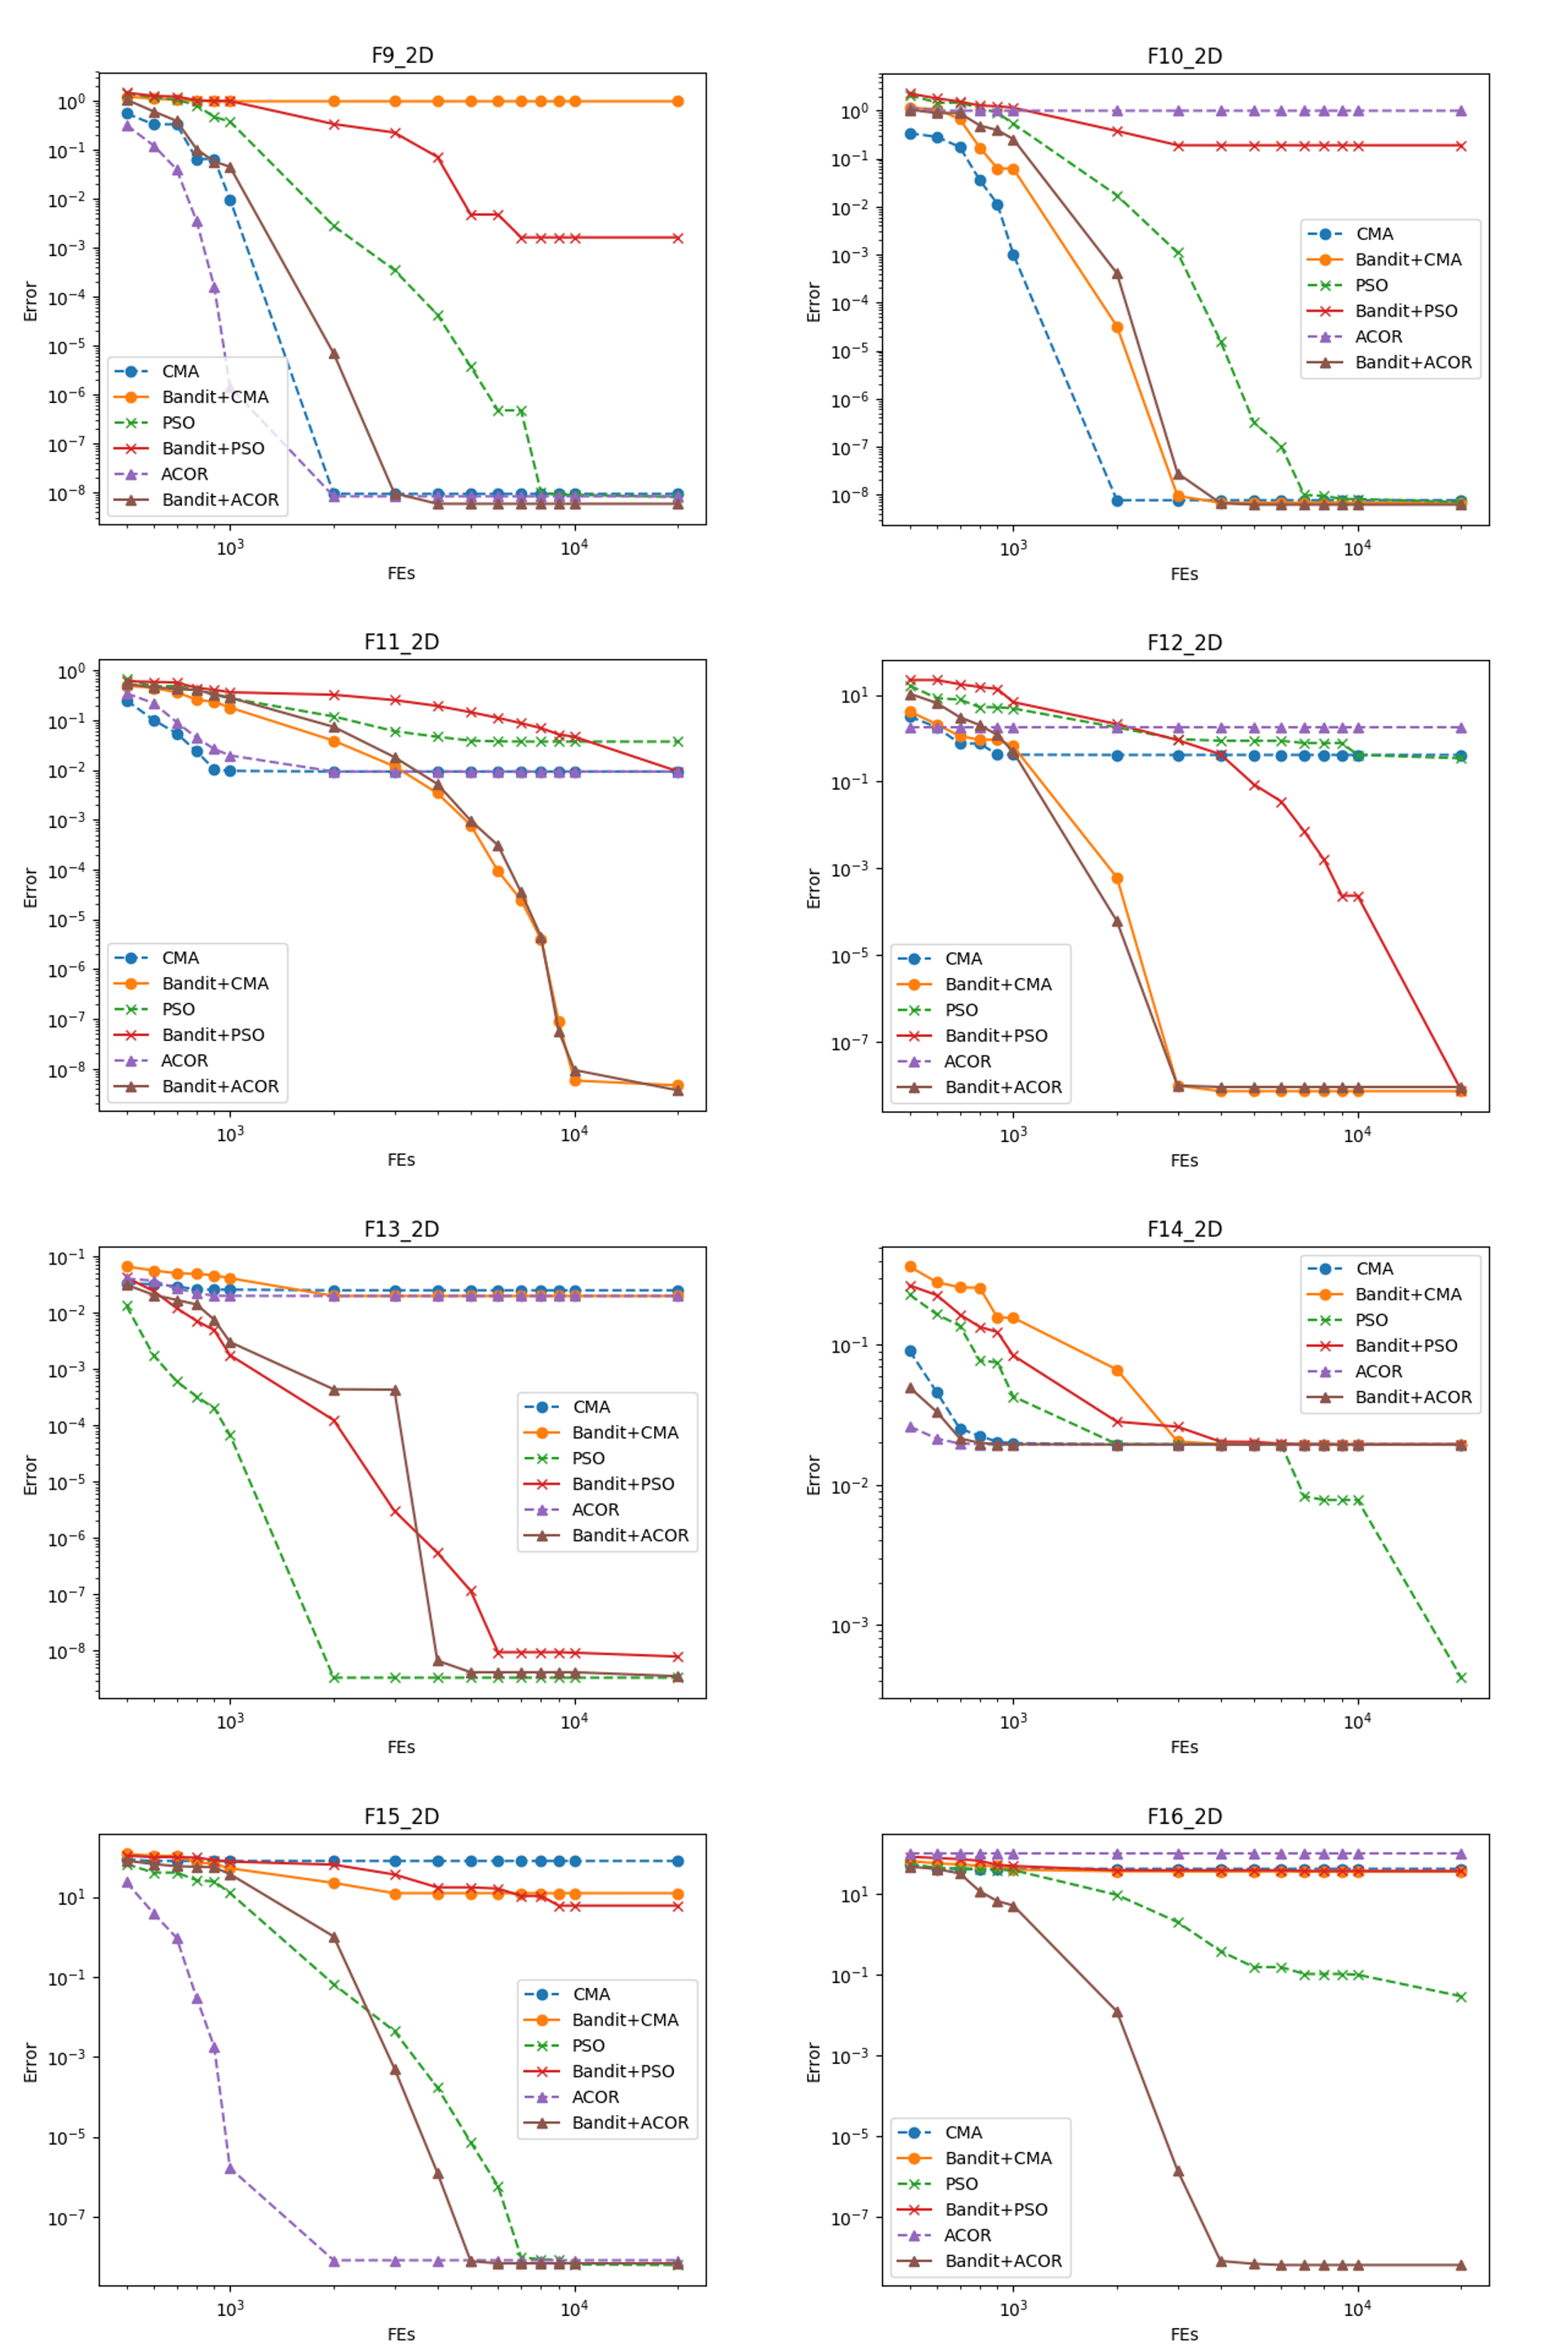
\includegraphics[width=\textwidth]{Median_F9_F16}
\caption{Median error of Problem 9 to Problem 16.}\label{fig:Median_F9_F16}
\end{figure}

\begin{figure}
\centering
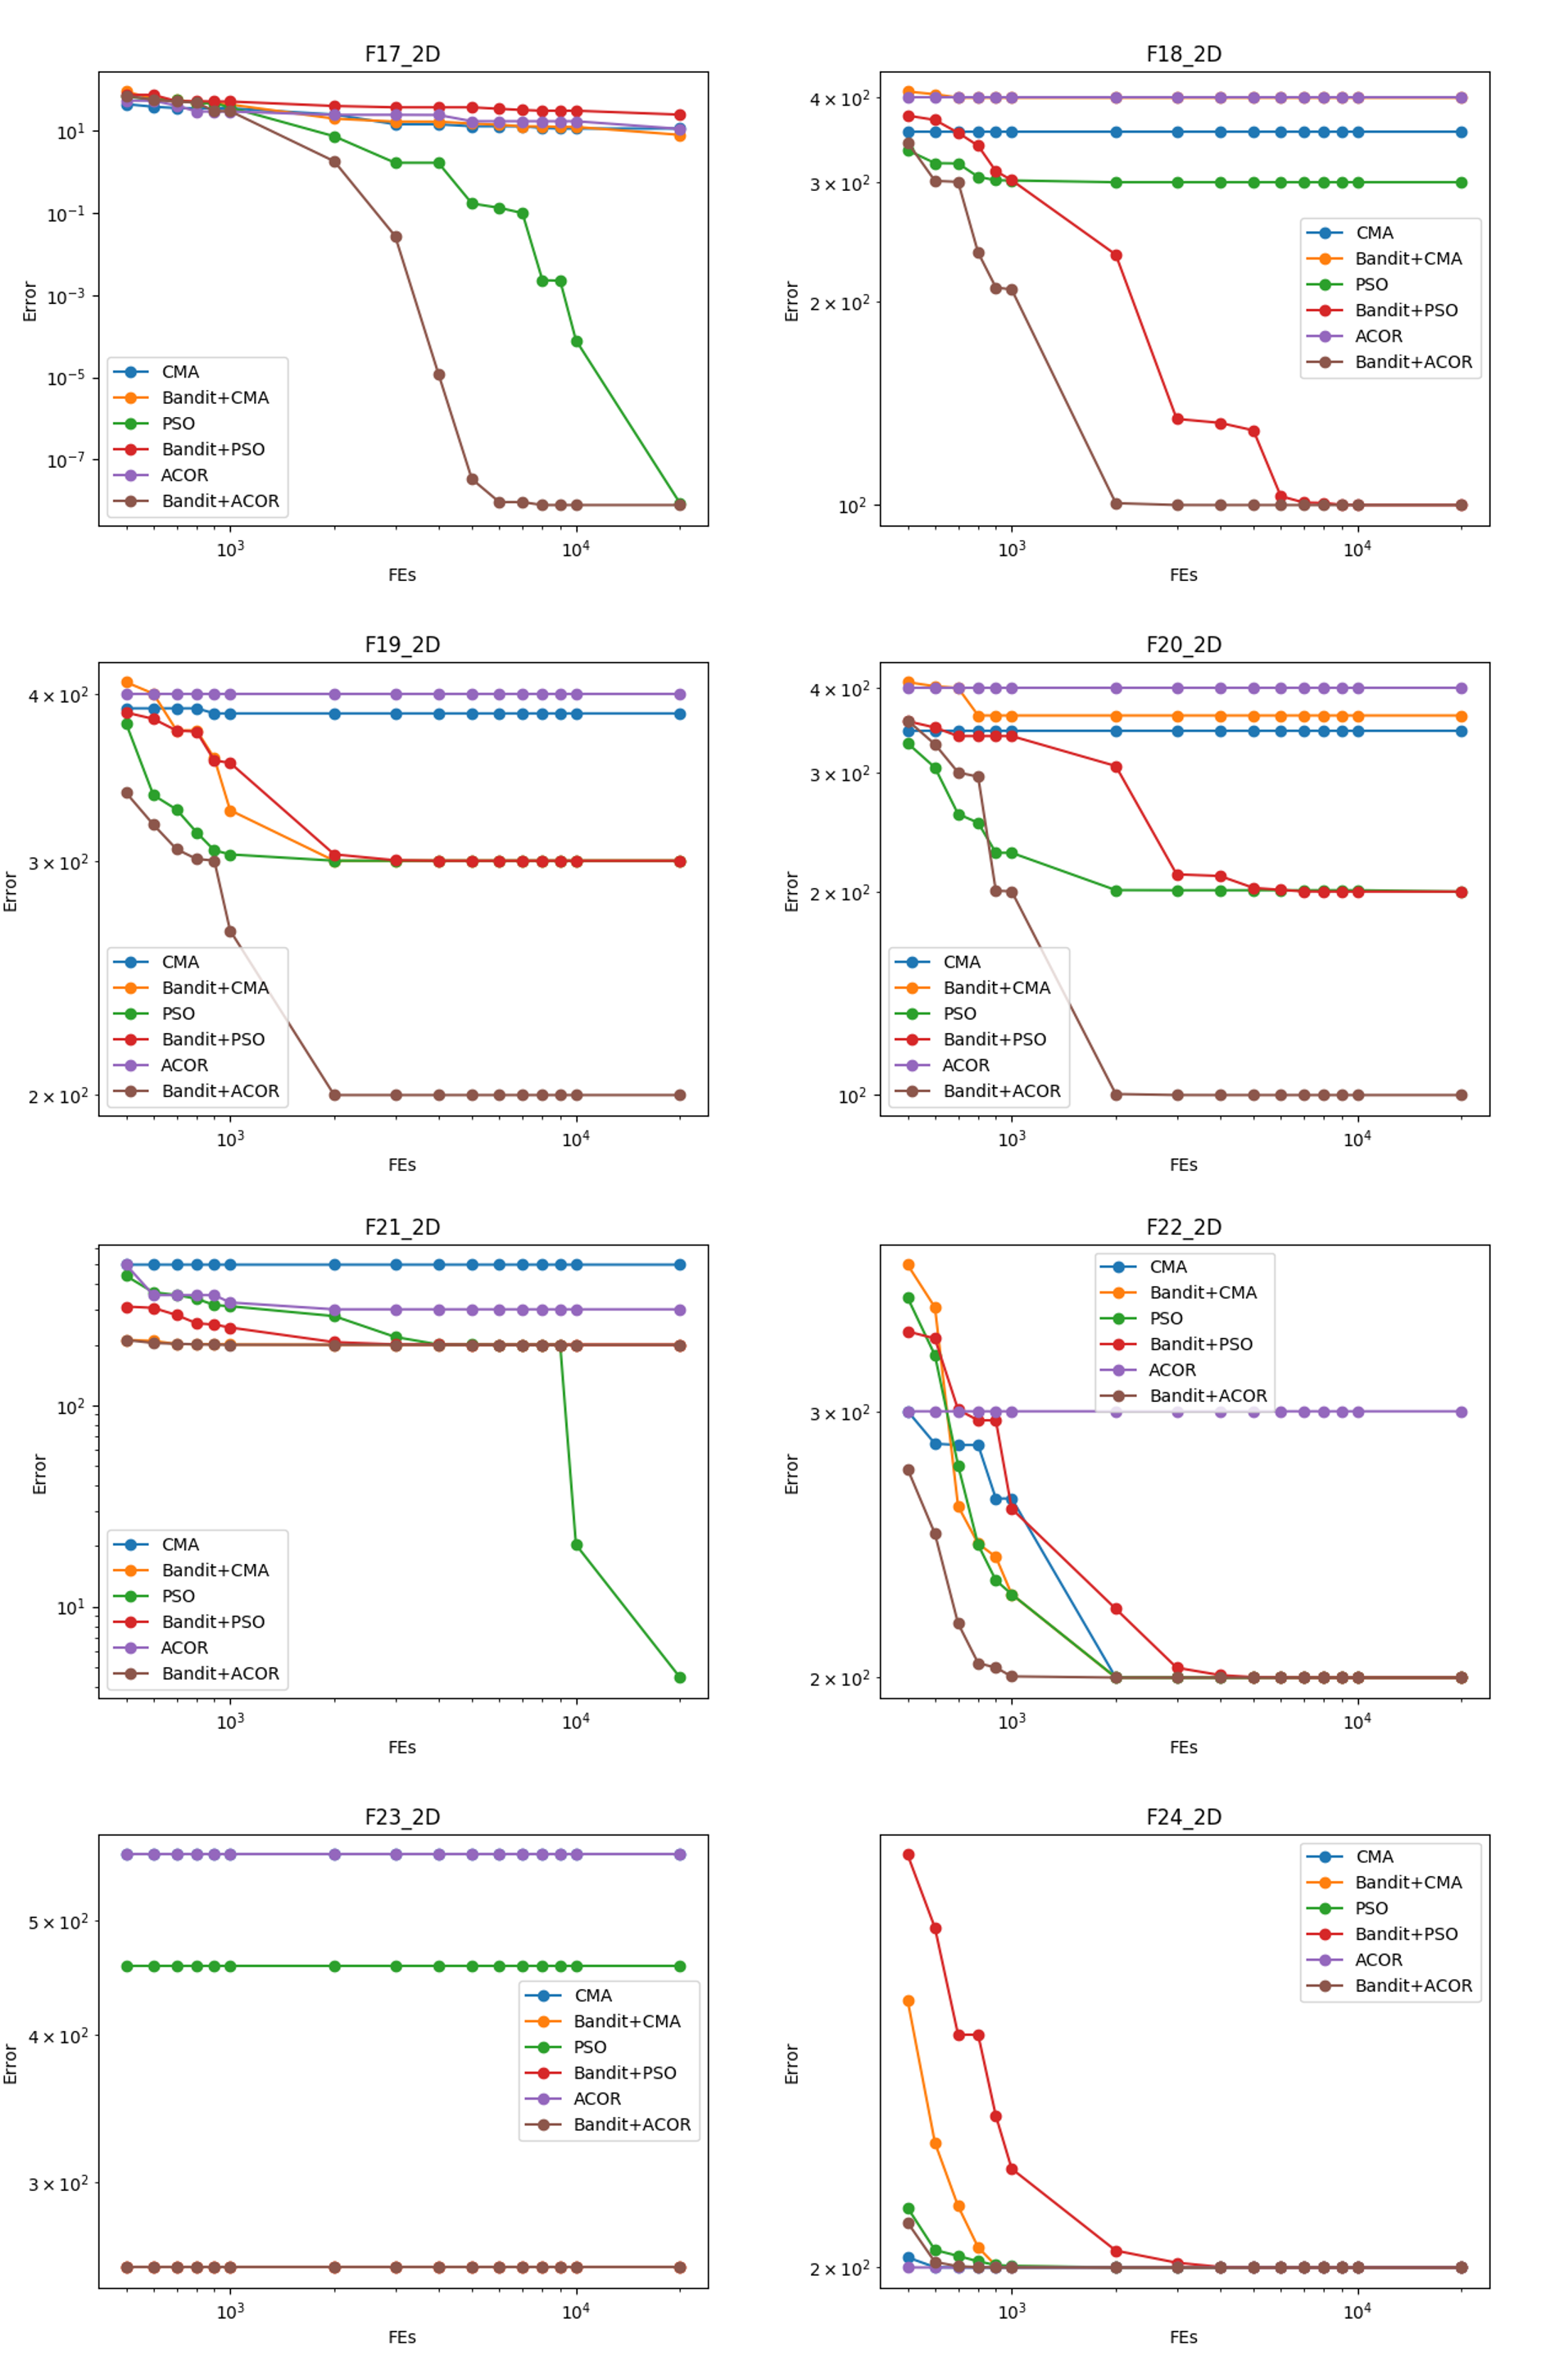
\includegraphics[width=\textwidth]{Median_F17_F24}
\caption{Median error of Problem 17 to Problem 24.}\label{fig:Median_F17_F24}
\end{figure}

\begin{figure}
\centering
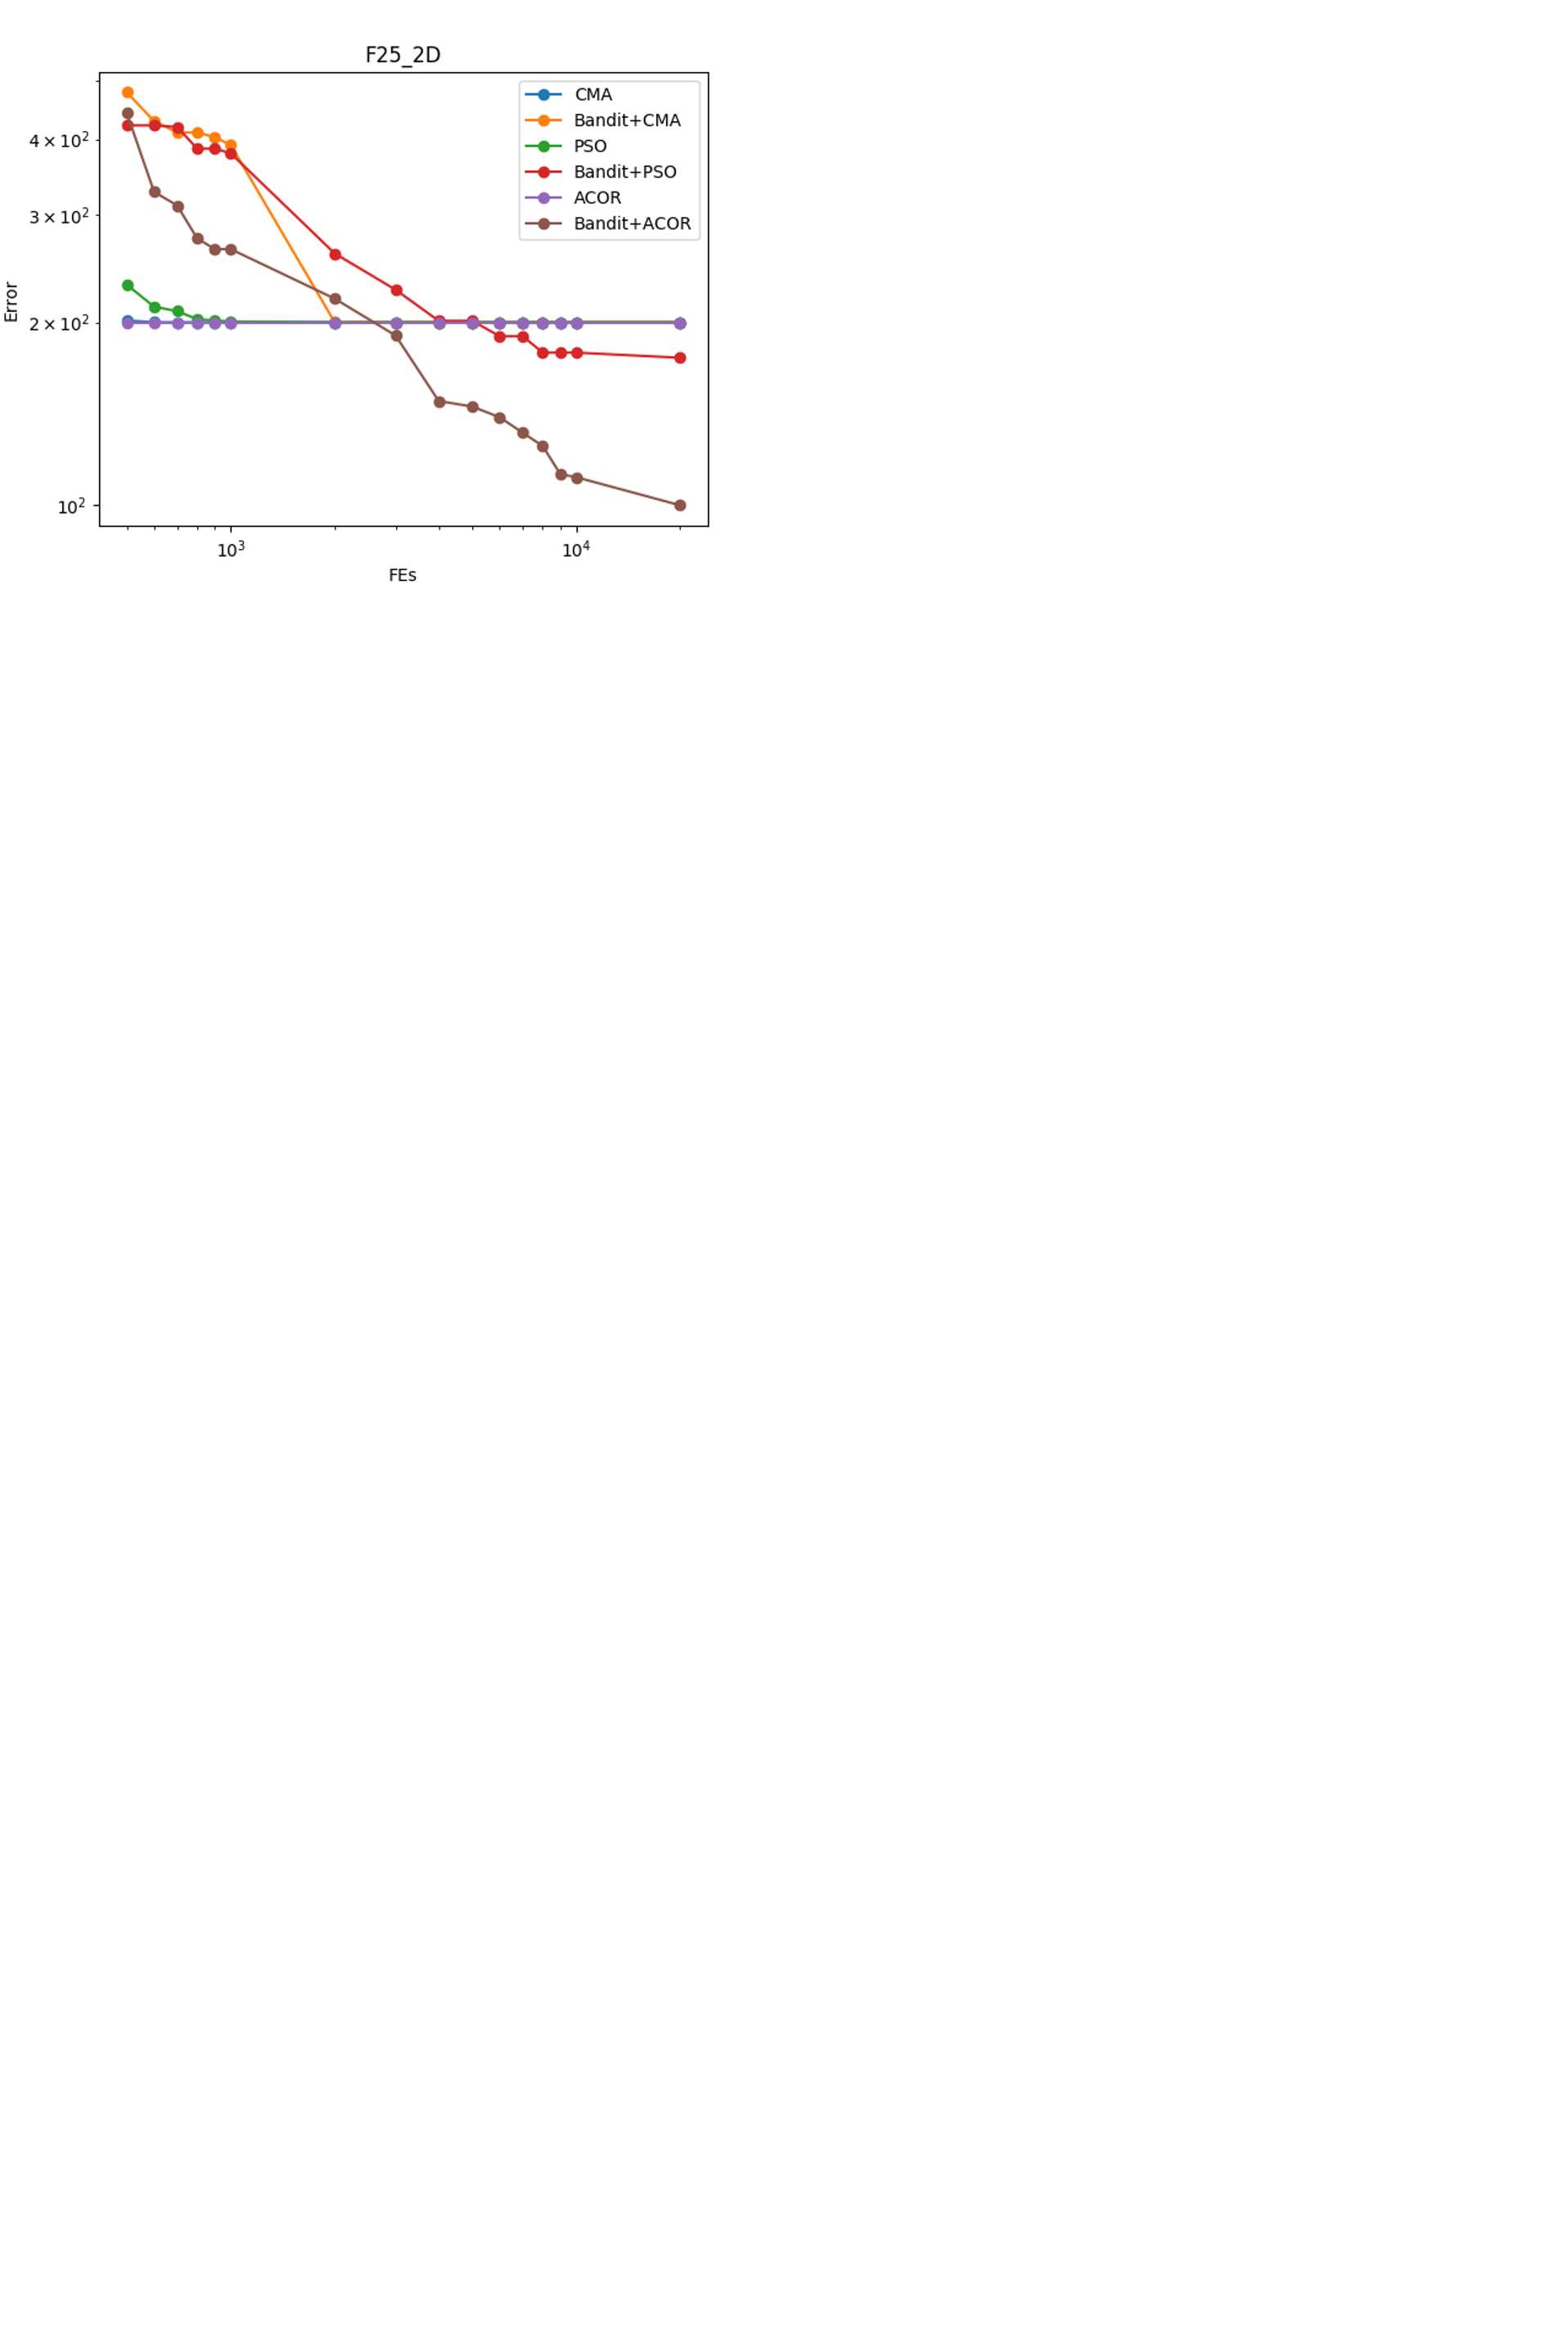
\includegraphics[width=\textwidth]{Median_F25}
\caption{Median error of Problem 25.}\label{fig:Median_F25}
\end{figure}


\chapter{Conclusion}
\label{chapter:conclusion}

In this thesis, we proposed a new multimodal optimization technique that aims to break down the multimodal problem into unimodal problems.
This technique is composed of three main components: unimodal detection, region of interest optimization and resource allocation.
We use the three techniques to dynamically isolate potential unimodals and enlarge a specific interesting region on the subspace for algorithms to search more thoroughly.
We also manage the ratio between exploration and exploitation according to the remaining resources,
so that the optimization process can be more efficient.

First, we proposed a unimodal detection technique to find potential \textit{fitness hills} in a real-valued multimodal problem 
by hierarchical clustering and Minimum Descriptioni Length.
It depicts the underlying \textit{fitness hills} better than K-Means.
Also unlike K-Means which needs to collaborate with other methods to determine the number of clusters,
our technique intrinsically detects the number of potential unimodals.

Second, we also proposed a method to seperate the search space into smaller subspaces in order to enhance performance.
We use linear projection matrix to project the search space to a subspace with well-defined boundaries for feasible solutions.
Therefore, the algorithm only needs to search within a hypercube, constrined by $[0,1]$ in all dimensions.
This technique is perferable for algorithms that requires a box-shape boundaries.
It also creates ROIs on the original search space that isolates the unimodals.
We also use the (1+1)-ES to optimize the projection matrix so that the ROIs have minimal-overlapping, thus enhance the searching efficiency.
By cracking down the original search space into multiple non-overlapping subspace, 
alogrithms now only have to search a smaller portion of the landscape which ideally consists of only one unimodal.

Furthermore, we proposed a new Multi-armed Bandit techniques that optimize the resource allocation.
We also explained how to maintain a more stablize cluster shapes during \textit{recluster}, 
yet still conserve the flexibility to split when needed.
We believe that in the beginning, when there are abundant of resources left, we should invest more resources in exploration.
That means we should update each clusters more equally for exploration.
Later, as the algorithms update the particles, we should be able to merge clusters to eliminate redundant search,
or split a cluster and invest more particles to search in a certain region.
When there are few evaluations left, we should concentrate on exploiting the current best hill.

However, there are still many issues that can be improved.
Our experiment results shows that there are still stability issues.
We need to investigate more on how to delete unnecessary arms.
Thus, this technique tends to cost more evaluations on problems 
that need to move for a long distance after converging to a relatively narrow valley.
Also, the clustering techniques to identify underlying unimodals can be further improved.
The current hierarchical clustering technique can be extended to a complete tree that contains all clusters.
Moreover, since this technique is composed of many relatively complex methods, 
speeding up computational time is also a crutial issue for all hyperparameters tuning techniques.






\backmatter

\addcontentsline{toc}{chapter}{\bibname}
\bibliographystyle{abbrv}

% Your bibliography goes here
\bibliography{thesis}

\appendix

\end{document}
